\documentclass[10pt,polish,a5paper,final,twoside,fleqn,onecolumn]{skryptzast}
\usepackage[top=1.5cm, bottom=1.5cm, left=1cm, right=1cm]{geometry}
\usepackage[utf8]{inputenc}
\usepackage[OT4]{fontenc}

\usepackage{tikz}
\usepackage{tikz-qtree}
\usepackage{enumitem}

\usepackage{datetime}
\usepackage{multicol}
\usepackage[widespace]{fourier}   % Use Utopia font set
\usepackage[scaled=0.875]{helvet} % Use Helvetica for sans-serif
\renewcommand{\ttdefault}{lmtt}   % Use Lucida Mono for monotype
\usepackage{booktabs}             % Booktabs for tables
\usepackage{multirow}
\usepackage{algorithm2e}
\usepackage{placeins}
\usepackage{amsmath}
\usepackage{graphicx} 
\usepackage{floatflt}
\usepackage{wrapfig}
\usepackage{xspace} 
\usepackage[style=long,nonumberlist]{glossaries}

\usepackage{amsthm} % pushQED, popQED
\newenvironment{aquote}[1]{%
  \pushQED{#1}%
  \begin{quote}
}{%
  \par\nointerlineskip\noindent\hfill(\popQED)%
  \end{quote}%
}

\title{Skrypt kursu zastępowych}
\author{Praca grupowa}
\date{data utworzenia: \today}

\hyphenation{hu-f-ce no-we lwo-wskim spa-do-chro-niar-stwo szy-ty m-o-ż-e} 

\begin{document}
\maketitle
\begin{figure}[h]
\centering
  
\includegraphics[width=6cm]{grafiki/lilijka.jpg}
\end{figure}
\bigskip 
\begin{center}
\textbf{ZHR}

III Poznański Hufiec Harcerzy ,,Horyzont''

Kurs Zastępowych \textbf{,,WSCHÓD I''}
\end{center}

\clearpage

\begin{aquote}{Robert Baden Powell}
Gdybym dziś mógł wybierać miejsce, które chciałbym zajmować w ruchu, to chciałbym być zastępowym.
\end{aquote}
 
\begin{aquote}{Roland E. Philipsl}
System zastępowy nie jest jedną z wielu metod organizowania pracy skautowej, lecz jest  on jedyną metodą.
\end{aquote}
\cleardoublepage
\pagenumbering{Roman}\pagestyle{skryptzast}%
\tableofcontents* \cleardoublepage%

\mainmatter
\chapter{Wstęp}

Czuwaj!
\begin{floatingfigure}[l]{3cm}
  
\includegraphics{grafiki/intro.png}
\end{floatingfigure}
Niniejszy skrypt zawiera informacje, które z pewnością przydadzą Ci się w prowadzeniu zastępu. Można go nazwać czymś w rodzaju ściągi. Nie bój się do niego zaglądać, gdy o czymś zapomnisz. Śmiało notuj i podkreślaj te elementy, które są dla Ciebie ważne. Wiedz, że Kurs Zastępowych "Wschód" oraz ten notatnik to tylko wparcie. Najważniejszy jesteś Ty, Twój zapał i chęć działania - to one sprawią, że Twoje zbiórki wyjątkowe a atmosfera w zastępie niepowtarzalna. 

Żeby być dobrym zastępowym, musisz być dobrym harcerzem. Pewnie zadałeś sobie pytanie, po co to całe harcerstwo? Trzeba wiedzieć po co coś robię i dlaczego. To są podstawy. Pamiętaj zatem: celemen naszego pobytu w ZHRze jest wychowywanie metodą harcerską --- w myśl przyrzeczenia i prawa harcerskiego dobrych ludzi. Wszystko inne jest  środkiem do osiągnięcia tego celu. Przypomnijmy sobie fundamenty i podstawy: prawo i przyrzeczenie harcerskie.



\textbf{Przyrzeczenie harcerskie}%wersja ZHR

Mam szczerą wolę całym życiem pełnić służbę Bogu i Polsce, nieść chętną pomoc bliźnim i być posłusznym Prawu Harcerskiemu.


\textbf{Prawo harcerskie}%wersja ZHR
\begin{enumerate}[noitemsep,nolistsep] 
\item Harcerz służy Bogu i Polsce i sumiennie spełnia swoje obowiązki.
\item Na słowie harcerza polegaj jak na Zawiszy.
\item Harcerz jest pożyteczny i niesie pomoc bliźnim.
\item Harcerz w każdym widzi bliźniego, a za brata uważa każdego innego harcerza.
\item Harcerz postępuje po rycersku.
\item Harcerz miłuje przyrodę i stara się ją poznać.
\item Harcerz jest karny i posłuszny rodzicom i wszystkim swoim przełożonym.
\item Harcerz jest zawsze pogodny.
\item Harcerz jest oszczędny i ofiarny.
\item Harcerz jest czysty w myśli, mowie i uczynkach, nie pali tytoniu i nie pije napojów alkoholowych.
\end{enumerate}


\chapter{Historia}
\section{Scauting}
\begin{floatingfigure}[r]{3cm}
\centering
  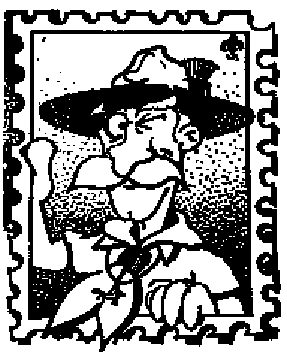
\includegraphics[width=3cm]{grafiki/bp.png}
\end{floatingfigure}
Twórcą skautingu jest gen. Robert Stephenson Smyth Baden - Powell. 
B-P urodził się w Londynie jako syn profesora na Uniwersytecie Oksfordzkim. 
To ten pogodny mężczyzna po lewej stronie. 
W dzieciństwie wiele czasu spędzał w gąszczu londyńskiego Hyde Parku, gdzie z pasją oddawał się podchodom. 
Wybierał się też często do dzielnic nędzy, rozmyślając o losie żyjących tam ludzi. 
Doszedł do wniosku, że tym, co najbardziej dzieli biednych od bogatych jest ich lichy strój, który pozwala na pierwszy rzut oka rozpoznać pochodzenie człowieka.

Jako młodzieniec skończył szkołą oficerską i rozpoczął służbę w Indiach. Będąc porucznikiem musiał szkolić rekrutów. 
Wkrótce zauważył, że kompania żołnierzy reaguje jak maszyna - obojętnie i bezmyślnie - i nie ma tu mowy o inicjatywie indywidualnej. 
Podzielił ją więc na patrole, a na dowódców wyznaczył najzdolniejszych żołnierzy. 
Pozwolił im popełniać błędy, by zachęcić ich do działania, lecz przestrzegał ich przed popełnieniem tego samego błędu dwa razy. Sam szkolił dowódców patroli, oni zaś - swoich żołnierzy. 
Później system ten zyskał uznanie i został wprowadzony w całym wojsku brytyjskim! 
Przebywając w Indiach wciąż jako porucznik doprowadził do wprowadzenia do armii nowego typu wywiadu, który został nazwany scoutingiem.

Zwiadowcy Baden-Powella początkowo byli namawiani do niepalenia, później niepalenie stało się warunkiem zostania zwiadowcą (zwiadowca musiał mieć sprawny \\ węch). 
Skuteczność scoutingu udowodnił, kiedy jego garnizon wygrał manewry z wojskami pułkownika Temple - właśnie dzięki nowym metodom wywiadowczym. 
Swoje metody oparł na obserwacjach hinduskich tropicieli i myśliwych oraz na własnych doświadczeniach z dziecięcych i młodzieńczych zabaw z braćmi. Wojsko poleciło mu napisać podręcznik, który nazwał Służba rozpoznania i łączności. 
Od tego czasu zajmował się szkoleniem zwiadowców. 
Niedługo potem w Afryce, już jako kapitan, B-P był świadkiem śmierci małej Zuluski, postrzelonej nieumyślnie przez wojsko. 
Później domagał się wprowadzenia do wojska szkolenia z zakresu pierwszej pomocy. 
Kierując budową drogi i mostów prowadzących przez dżunglę do pewnej twierdzy, zauważył, że wśród pracujących dla niego tubylców pewna część wyróżniała się. 
Ci ludzie witali się przez podawanie sobie lewej ręki. 
Okazało się, że stanowią oni pewien rodzaj elity wśród swojego plemienia. Ich powitanie stało się później powitaniem wszystkich skautów. 
Udoskonalał wciąż metody zwiadowcze, opierając się na obserwacji afrykańskich wojowników. Wydał nowy podręcznik wojskowy Poradnik scoutingu.

Bardzo ważnym wydarzeniem była obrona Mafekingu przed wojskami burskimi. Baden - Powell jako pułkownik dowodził dziesięciokrotnie mniejszym oddziałem od wojsk oblężniczych. 
\begin{wrapfigure}{r}{3cm}
  \begin{center}
    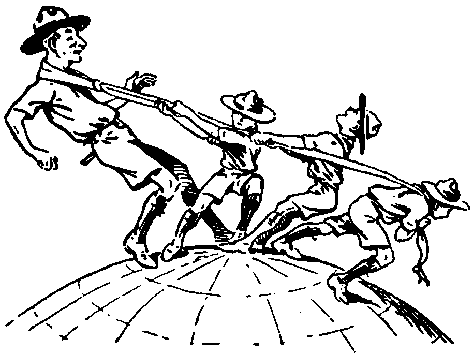
\includegraphics[width=2.9cm]{grafiki/bardzo.png}
  \end{center}
\end{wrapfigure}
Musiał więc do służby zaangażować także młodych chłopców. Zadziwiło go, że sprawowali się oni w sposób nadspodziewanie odpowiedzialny. Doszedł do wniosku, że chłopiec, który dostanie odpowiedzialne zadanie, spełni je niejednokrotnie lepiej od regularnego żołnierza. Obrona Mafekingu dzięki nieziemskiemu sprytowi Baden-Powella zakończyła się sukcesem Brytyjczyków. B-P jeszcze przed powrotem do Anglii usłyszał od brata, który przybył do Mafekingu jako major, interesującą wiadomość. Mianowicie, jego drugi podręcznik Poradnik skautingu, który był obowiązkową lekturą każdego żołnierza, zyskał niesamowitą popularność wśród młodzieży. Według relacji brata młodzi chłopcy masowo wyjeżdżali za miasto i tam odbywali wędrówki wykorzystując całą wiedzę zawartą w podręczniku B-P. On sam zawsze zadawał sobie pytanie jak uniknąć wojen. I wydało mu się, że teraz znalazł klucz, że wzrastający w obcowaniu z przyrodą młodzi chłopcy wyrastają na innych ludzi niż ci tkwiący w wielkim mieście, że gry na orientację wyrabiają postawę dążenia do celu, co odbije się postawą konsekwencji w dorosłym życiu.

B-P wrócił do Londynu jako bohater i wyzyskując sprzyjającą sytuację zajął się organizacją ruchu młodzieżowego, który nazwał skautingiem. Na jego kształt wpłynęły opisane fakty z jego życia: opierał się na systemie małych grup (zastępy), kontakcie z przyrodą, powierzaniu odpowiedzialności młodym ludziom. Wprowadził do niego szkolenie pierwszej pomocy i mundur, który zacierał różnice między biednymi i bogatymi. Przeredagował też swój wojskowy podręcznik tak, by mógł służyć młodzieży i wydał go pod nazwą Skauting dla chłopców. Organizacją ruchu skautowego zrealizował także swoje dawne marzenie zmiany surowego wiktoriańskiego modelu wychowania. Pierwszy obóz skautowy odbył się w 1907 roku na wyspie Brownsea u wybrzeża Wielkiej Brytanii w okolicy portu Poole. W 1909 roku w Anglii odbył się pierwszy zlot skautowy z udziałem 11.000 uczestników. W 1912 ukazał się pierwszy żeński podręcznik skautowy. W 1920 w Londynie odbył się I Zlot Międzynarodowy Jamboree . B-P został na nim uznany przez wszystkie światowe organizacje skautowe Skautem Naczelnym Świata. Przez ojczyznę został obdarzony tytułem lorda. B-P zmarł w 1941 roku w Kenii. 

\section{Powstanie harcerstwa w Polsce. harcerstwo w II Rzeczypospolitej}

Jesienią 1909 roku niemal jednocześnie w dwóch czasopismach (warszawskim i lwowskim) ukazały się artykuły informacyjne o nowym ruchu wychowawczym, który zdobył sobie niezwykłą popularność wśród młodzieży angielskiej (mowa o skautingu). Metody skautowe zwróciły uwagę działaczy Zarzewia (Henryk Bagiński, Andrzej Małkowski – to ten po lewej, Neugebauer) - tajnej młodzieżowej organizacji paramilitarnej przygotowującej swych członków do walki o niepodległość Polski.\begin{wrapfigure}{l}{3cm}
  \begin{center}
    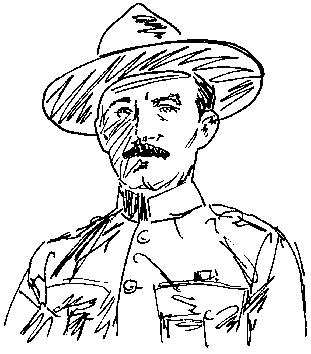
\includegraphics[width=2.9cm]{grafiki/malkowski.png}
  \end{center}
\end{wrapfigure} Władze Zarzewia zleciły Andrzejowi Małkowskiemu przetłumaczenie angielskiego podręcznika Scouting for boys. Szybko stał się on entuzjastą skautingu, uważając go za nowy styl życia.
Małkowski był także członkiem towarzystwa gimnastycznego Sokół we Lwowie - potężnej wówczas organizacji, jawnej, działającej w trzech zaborach (w rosyjskim tajnej), mającej własną sieć sal gimnastycznych. Był również członkiem Stowarzyszenia Eleusis propagującego poczwórną wstrzemięźliwość - od alkoholu  i tytoniu. To właśnie tej organizacji zawdzięczamy 10. punkt Prawa Harcerskiego, ewenement na skalę światową oraz patriotyczno-narodowy charakter harcerstwa. Małkowski wciągnął do współpracy innych członków tego stowarzyszenia - Wincentego Lutosławskiego, Tadeusza Strumiłłę, Jerzego Grodyńskiego, Jadwigę Falkowską, Olgę Drahonowską (swoją przyszłą żonę) i wielu innych. Zarzewiacy, elsowie, wszyscy uczestnicy kursu chłonęli informacje o skautingu. 21. maja 1911 r. powstała Komenda Skautowa we Lwowie. W dzień później A. Małkowski wydał rozkaz o powołaniu pierwszych drużyn: trzech męskich i jednej żeńskiej. W lipcu 1911 r. ukazała się pierwsza polska książka skautowa: Skauting jako system wychowania młodzieży na podstawie gen. Roberta Baden-Powella <<Scouting for boys>> przedstawił Andrzej Małkowski. 15. października wyszedł we Lwowie pierwszy numer dwutygodnika Skaut z wierszem Wszystko co nasze... na stronie tytułowej, redagowany przez Małkowskiego. Na bibułach (powszechnie stosowaną konspiracyjną metodą), podobnie jak książka Małkowskiego, Skaut docierał do wszystkich zaborów. Skauting ze Lwowa promieniował na cały, choć podzielony, kraj. W grudniu utworzono w Warszawie Naczelną Komendę Skautową na Królestwo Polskie (część zaboru rosyjskiego).

W lutym 1912 roku na łamach Skauta rozstrzygnięty został konkurs na polską odznakę skautową, ogłoszony w jego pierwszym numerze. Żadna z prac nie wydała się na tyle interesująca, by od razu wprowadzić ją do użytku, toteż w końcu roku NKS wyznaczyła do dalszych prac nad projektem ks. Kazimierza Lutosławskiego z zespołem, którego praca zdobyła w konkursie III nagrodę. Jego projekt wzorowany był na orderze Virtuti Militari. Po wprowadzeniu w nim szeregu zmian, Krzyż Harcerski zaprojektowany przez ks. Lutosławskiego wszedł do użytku w 1913 roku. To właśnie na nim po raz pierwszy w Polsce znalazła się lilijka harcerska, wzorowana na lilijce skautowej. 24 - 25 marca 1912 roku odbył się pierwszy zjazd drużyn i plutonów harcerskich. Przybyło na niego 100 uczestników. W czerwcu 1912 ukazała się znana polska książka Eugeniusza Piaseckiego i Mieczysława Schreibera Harce młodzieży polskiej, w której po raz pierwszy użyto staropolskiej terminologii rycerskiej, czyli wyrazów takich, jak: harcerz (zastąpił określenie skaut polski), zastęp (zastąpił określenie pluton), drużyna, hufiec, harce (oznaczające kiedyś ćwiczenia rycerstwa przed bitwą). Zaproponowano w niej także używane do dziś nazwy stopni i funkcji (wyraz chorągiew również należy do dawnej terminologii rycerskiej).

2. lipca 1913 roku 43 skautów z trzech zaborów wyjechało na III Wszechbrytyjski Zlot Skautów w Birmingham. Mieli tam obóz pod polską flagą! Tuż przed wybuchem I wojny światowej polski skauting liczył ponad 15.000 członków. Już wtedy tworzono polskie harcerstwo poza (wtedy jeszcze historycznymi) granicami kraju. Podczas całej wojny skauci brali udział w bardzo wielu akcjach pomocniczych i zbrojnych. Konflikty polityczne spowodowane wybuchem wojny podzieliły skautów na kilka organizacji. Jednak w Królestwie Polskim wobec utrudniania działalności harcerstwa przez władze, organizacje harcerskie postanowiły się zjednoczyć. 1 i 2 listopada 1916 roku w Warszawie w efekcie zjednoczenia wszystkich organizacji harcerskich zaboru rosyjskiego powstaje Związek Harcerstwa Polskiego. Do zjednoczenia harcerstwa wszystkich zaborów doszło na zjeździe w Lublinie 1 i 2 listopada 1918 roku, gdy na ulicach miast rozpoczęło się już rozbrajanie wrogich wojsk. Oficjalnie przyjęto na nim nazewnictwo zaproponowane przez Piaseckiego i Schreibera. Harcerstwo liczyło wtedy już ok. 30~000 członków. W nocy z 15 na 16 stycznia 1919 roku w katastrofie morskiej w Cieśninie Messyńskiej zginął Andrzej Małkowski. Od 31. grudnia 1920 do 2. stycznia 1921 roku obradował w Warszawie I Walny Zjazd ZHP, na którym przyjęto statut ZHP. 
\begin{wrapfigure}{l}{3cm}
  \begin{center}
    
\includegraphics[width=2.9cm]{grafiki/lipca.png}
  \end{center}
\end{wrapfigure}
4 - 9 lipca 1924 odbyły się pierwsze narodowe zloty: harcerzy na Siekierkach i harcerek w Świdrze. Po odzyskaniu niepodległości zwrócono uwagę na dominujący, nadmiernie rozbudowany w harcerstwie militaryzm, który wówczas nie był już potrzebny. Szukano sposobu wyjścia z kryzysu. Stworzono więc programy specjalnościowe, które okazały się świetnym na niego lekarstwem. Rozwijało się harcerskie szybownictwo, żeglarstwo, kajakarstwo, turystyka kwalifikowana, krótkofalarstwo, strzelectwo, spadochroniarstwo, rozmaite kluby sportowe. Harcerstwo kwitło dzięki dużemu wsparciu finansowemu państwa. Punktem kulminacyjnym jego rozwoju okazał się słynny zlot w Spale 11 - 27 lipca 1935 roku. Wzięło w nim udział 25~000 uczestników. Wcześniej, poczynając od 1933 roku, Aleksander Kamiński rozpoczął rozwój zuchostwa. Choć pierwszą drużynę zorganizowała w 1914 roku w Zakopanem Olga Małkowska, wzorując się na brytyjskich Wilczętach, dopiero Kamiński znalazł odpowiednie rozwiązania metodyczne i uczynił z ruchu zuchowego poważną gałąź działalności harcerstwa. W końcu 1938 roku dwie części składowe ZHP - Organizacja Harcerzy i Organizacja Harcerek liczyły odpowiednio 130~500 i 71~600 członków. We wrześniu 1938 roku w związku z akcją zajęcia przez wojsko polskie Zaolzia utworzono Pogotowie Harcerek z odrębną siecią podległości pod komendanturą hm. Józefiny Łapińskiej. Po zakończeniu operacji nie zostało ono zlikwidowane. Trwały szkolenia sanitarne, łącznościowe, przeciwlotnicze i przeciwgazowe.

\section{Harcerstwo podczas II wojny światowej}

Wiele było przykładów udziału harcerzy w działaniach wojennych Kampanii Wrześniowej. U jej kresu, 27 września 1939 roku w Warszawie (w dniu jej kapitulacji), na naradzie obecnych w Warszawie członków Naczelnej Rady Harcerskiej i innych wybitnych instruktorów zapadła decyzja o kontynuowaniu działalności harcerstwa w konspiracji. Naczelnikiem harcerstwa męskiego wybrano hm. Floriana Marciniaka (ps. Nowak), który miał je zorganizować i stworzyć jego program, przyjmując dla niego kryptonim Szarych Szeregów. Kryptonimy jednostek organizacyjnych były następujące: Kwatera Główna - Pasieka, chorągwie - Ule, hufce - Roje, drużyny - Rodziny, zastępy - Pszczoły. Harcerki miały działać w zorganizowanym już Pogotowiu Harcerek, które występowało pod kryptonimem Związek Koniczyn, Szare Szeregi żeńskie, a później Bądź gotów. Część dziewcząt działało w organizacji męskiej w rozmaitych służbach pomocniczych oddziałów, a zwłaszcza w służbach sanitarnej i łączności. W wyżej wymienionych oraz w różnych służbach cywilnych (opieka nad dziećmi, pomoc więźniom, jeńcom i ich rodzinom, pomoc ludziom starym i chorym, Żydom, tajne nauczanie) działało Pogotowie Harcerek, a później Związek Koniczyn. Pełniły one te funkcje zarówno we wrześniu 1939 r., w czasie okupacji, jak i podczas Powstania Warszawskiego. Gdy w lutym 1942 roku powstał Referat Wojskowej Służby Kobiet AK (a była ona organizowana już od października 1939), harcerki powyżej 16 lat były przekazywane do jego dyspozycji. Zastępczyniami komendantki WSK były instruktorki harcerskie - Jadwiga Falkowska i Ewa Grodecka. Pierwszym zadaniem dowództwa Szarych Szeregów była konsolidacja oraz integracja organizacji, istniało bowiem wiele realizujących własny program drużyn, wiele związało się z mnożącymi się wówczas tajnymi organizacjami (między innymi słynna później szaroszeregowa 23. WDH Pomarańczarnia Zośki). Aby wyeliminować problem masowego odchodzenia starszych harcerzy do oddziałów wojskowych, organizowano im uczestnictwo w szkoleniach i służbach Związku Walki Zbrojnej (późniejszej Armii Krajowej) nie zmieniając ich przynależności organizacyjnej. Kłopotem był brak szkolnictwa ponadpodstawowego, przez co młodzież organizowała się w kręgi samokształceniowe stanowiące konkurencję dla harcerstwa.

W grudniu 1940 roku Aleksander Kamiński sformułował program akcji Wawer, który znalazł szeroki odzew wśród całej, nie tylko harcerskiej, młodzieży (poza organizacją nawet wśród dzieci). 
Nazwa pochodziła od nazwy podwarszawskiej wówczas miejscowości, gdzie w grudniu 1939 roku okupant dokonał pierwszej masowej zbrodni w rejonie Warszawy mordując ponad 100 ludzi wywleczonych z domów w odwecie za śmierć niemieckiego żołnierza zamordowanego przez kryminalistów. 
\begin{wrapfigure}{l}{3cm}
  \begin{center}
    
\includegraphics[width=2.9cm]{grafiki/onc.png}
  \end{center}
\end{wrapfigure}Dla warszawiaków nazwa ta wyrażała nienawiść do najeźdźcy. Początkowo Wawer polegał na płataniu figli, częstokroć bardzo dokuczliwych, Niemcom i polskim zdrajcom (szykany, napisy na murach, ulotki, wybijanie szyb). Później mały sabotaż podejmował także trudniejsze zadania - gazowanie kin, wywieszanie polskich flag, nadawanie polskich audycji przez niemiecką sieć radiową, kolportaż polskich dodatków do wydawanej przez Niemców prasy, rozmaite akcje propagandowe. Akcja Wawer w ciągu całego roku 1941 znacząco przyczyniła się do pokonania problemów Szarych Szeregów, z czasem przestała jednak wystarczać starszej młodzieży. Jej wejściu do struktur wojskowych sprzyjało przekształcenie ZWZ w AK, gdzie zaszły istotne zmiany w formach i kierunkach działania wojska. Po uregulowaniu stosunku Sz. Sz. i AK (rozkaz Komendanta Głównego AK z marca 1942 r.) starsza młodzież miała współistnieć jednocześnie w obu organizacjach, młodsza miała brać udział jedynie w szkoleniach i służyć w służbach pomocniczych. W połowie 1942 roku wprowadzono ostatecznie program Sz. Sz. Dziś – Jutro - Pojutrze. Dziś oznaczoło walkę konspiracyjną, Jutro - powstanie, Pojutrze - wolną Polskę. Każda z wyodrębnionych wkrótce grup wiekowych w inny sposób realizowała walkę Dziś oraz przygotowywała się do walki Jutro i pracy w wolnej Polsce Pojutrze. Pojutrze miało zapobiegać całkowitej militaryzacji młodzieży, sprawić, aby była ona gotowa do życia w kraju po wojnie, aby wojna nie zrobiła z niej wraków niezdolnych do życia w normalnych warunkach. Zawiszacy realizowali lżejsze formy akcji Wawer, rozprowadzali prasę, zajmowali się łatwiejszymi formami łączności i wywiadu (na Dziś), byli szkoleni do służby pomocniczej (na Jutro) oraz uczyli się w szkole, oprócz niemieckiej podstawówki na tajnych kompletach uczyli się nieobecnych w niej przedmiotów: języka polskiego, geografii, historii; starsze roczniki uczyły się w szkołach zawodowych lub/i w tajnych gimnazjach, ponieważ Niemcy zlikwidowali całe szkolnictwo średnie poza szkołami zawodowymi (na Pojutrze).
\begin{wrapfigure}{r}{3cm}
  \begin{center}
    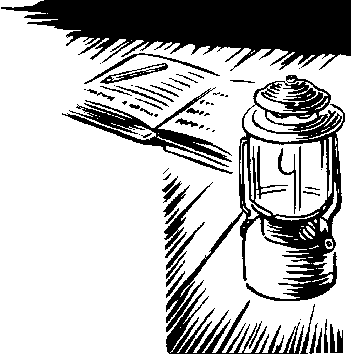
\includegraphics[width=2.9cm]{grafiki/rudy.png}
  \end{center}
\end{wrapfigure}
23 marca zaszła jednak konieczność przeprowadzenia akcji innego typu - aresztowano Rudego (Jana Bytnara), komendanta hufca Południe. Akcja ta, zupełnie precedensowa w skali całej AK, odbyła się 26. marca (17.30 - 17.45) i stała się pierwowzorem dla wszystkich późniejszych akcji dywersji miejskiej. Mimo swej niedoskonałości organizacyjnej (zespół wykonawczy liczył aż 28 osób) stanowiła przełom w sposobach walki z okupantem. Wcześniejsza próba jej przeprowadzenia nie była możliwa, ponieważ brakowało koniecznej decyzji nieobecnego w Warszawie mjr. Lipińskiego. W wyniku akcji zmarli Hubert (Hubert Lenk), Alek (Aleksy Dawidowski) i Buzdygan (Tadeusz Krzyżewicz). Zmarł także odbity Rudy, uwolniono również 23 innych więźniów. W 1944 roku było 18 chorągwi harcerzy (10 000 członków) i 14 chorągwi harcerek (5 000 członkiń). Do tych liczb trzeba dodać harcerzy ze środowisk działających niezależnie od kontynuatorów ZHP (drużyny samodzielne, inne organizacje). Wielu harcerzy zginęło w czasie II wojny światowej, a szczególnym miejscem, masowym grobem było Powstanie Warszawskie. To twoi starsi bracia, pamiętaj o nich. Konspiracyjne harcerstwo było ewenementem na skalę europejską. Trzecim i ostatnim naczelnikiem Sz. Sz. był Leon Marszałek, pełniący tę funkcję od października 1944 (Orsza dostał się wtedy do niewoli niemieckiej) do stycznia 1945 roku (gdy Armia Czerwona wkroczyła do Warszawy). Również w czasie wojny działało harcerstwo poza granicami kraju.

\section{Harcerstwo w PRL i w III Rzeczypospolitej}

Harcerstwo odradzało się żywiołowo w latach 1944 - 45 wszędzie tam, skąd Armia Czerwona wyparła Niemców. Ujawniały się lub powstawały drużyny, organizowały hufce i chorągwie. Wszystko to odbywało się oddolnie, jako że oficjalnie ZHP został powołany do życia decyzją władz oświatowych dopiero 30. grudnia 1944 roku. Nowe władze zdawały sobie sprawę z przydatności ZHP w wychowaniu dzieci i młodzieży, wiedziały jednak dobrze, że jest ono zdominowane przez siły im nieprzychylne, związane z rządem emigracyjnym i AK. Rozpoczęła się więc walka o harcerstwo. Władze utworzyły Tymczasową Naczelną Radę Harcerską, która przygotowała nowe Prawo i Przyrzeczenie oraz Deklarację Ideową. Rekonstrukcja władz centralnych nastąpiła w maju 1945 roku. Nastąpił duży dopływ dawnych instruktorów. Metody pracy opierały się na przedwojennych, a jej płaszczyzny były wynikały z ówczesnej sytuacji kraju: odgruzowanie, służba dla frontu, pomoc rannym, usuwanie pozostałości poniemieckich, pomoc przy żniwach, służba dziecku, pomoc repatriantom, praca dla Ziem Odzyskanych. Harcerstwo liczyło w lipcu 1945 roku ponad 200 000 członków. \begin{wrapfigure}{r}{2cm}
  \begin{center}
    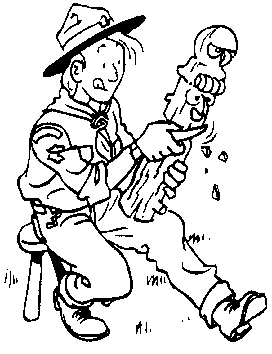
\includegraphics[width=1.94cm]{grafiki/str.png}
  \end{center}
\end{wrapfigure}
Nowych harcerzy przyciągała legenda Szarych Szeregów, jednak dużym problemem był brak kadry - na jednego instruktora przypadało wtedy 450 harcerzy. Był to czas rozwoju harcerskich instytucji zapewniających samowystarczalność - Centrali Dostaw Harcerskich, harcerskich warsztatów wytwarzających umundurowanie. Władze nie zezwalały na Walny Zjazd, gdyż żywiły słuszne obawy, iż zdecydowaną większość będą na nim mieli instruktorzy nie akceptujący władzy przyniesionej do Polski na bagnetach Armii Czerwonej. Starały się o rozszerzenie swych wpływów w ZHP. Wobec trudności z tym związanych, rozpoczęły ofensywę. Jednak starcia na górze w niewielkim stopniu docierały do drużyn.

W końcu 1947 roku Sekretarz Generalny ZHP Pelagia Lewińska przedstawiła projekt zmian organizacyjnych w Związku. Przejawem koncepcji centralnego sterowania programem drużyn była Harcerska Służba Polsce. 
Rezygnując z pracy indywidualnej, podejmowała ona rozmaite zadania społeczne skupione w 4 grupach: Las i rola, Kultura i oświata, Odbudowa kraju oraz Zdrowie i dziecko.
Organizacja rozwijała się liczebnie - w 1948 roku liczyła już 295 500 członków.

Konferencja komendantów i komendantek chorągwi, która odbyła się w dniach 18 - 20 grudnia, przyjęła uchwałę, w której stwierdziła, że obecni na niej instruktorzy zrywają z tradycją harcerską. Odpowiedzią na nią było odejście z ZHP kolejnej grupy instruktorów.

\begin{wrapfigure}{l}{3cm}
  \begin{center}
    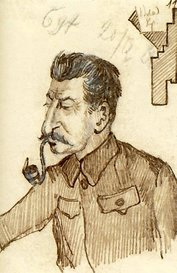
\includegraphics[width=2.9cm]{grafiki/stalin.jpg}
  \end{center}
\end{wrapfigure}
W latach 1848 - 49 zlikwidowano w Polsce wiele organizacji społecznych. Władze uznały, że ZHP jest w swojej obecnej formule nie do zaakceptowania. Postanowiono jednak wykorzystać pozytywny społeczny wizerunek harcerstwa. W styczniu 1949 ograniczono wiek młodzieży harcerskiej do 15 lat. Kontrolę nad ZHP przejmować zaczął Związek Młodzieży Polskiej. W sierpniu Pelagia Lewińska wydała broszurę Walka o nowe harcerstwo, w której oskarżała Związek o służbę na korzyść imperializmu, co było wówczas bardzo poważnym zarzutem. Usuwano kolejnych niewygodnych instruktorów. Na początku 1950 roku Zarząd Główny ZMP, któremu Prezydium przyznano stopnie harcmistrzów, podjął decyzję o przejęciu kierownictwa nad ZHP i ustalił termin jego wcielenia do ZMP na 15 października. Zmieniono Prawo i Przyrzeczenie, symbolikę i mundur. Odrzucono tradycyjne metodykę, formy pracy, rozwiązania programowe i organizacyjne. Zlikwidowano drużyny w szkołach średnich - po ukończeniu podstawówki, harcerze mieli przechodzić do podstawowych struktur ZMP. Odsunięto większość doświadczonych instruktorów. Przewodnikami drużyn zostali etatowi pracownicy szkół. Drużyna skupiała młodzież całej szkoły, a zastępy i ich odpowiedniki - ogniwa - odpowiadały klasie. Organizacja Harcerska ZMP wzorowana była na radzieckiej Organizacji Pionierskiej im. Włodzimierza Lenina, nie uwzględniono jednak odmienności polskich warunków. Harcerze podejmowali prace społeczne, uczestniczyli w wielkich konkursach i imprezach. Zastępy prowadzili nauczyciele, zbiórkami bywały lekcje, a na jednego przewodnika przypadało kilkuset uczniów. Dało to w sumie mało atrakcyjne zbiórki zupełnie nie uwzględniające potrzeb dzieci i młodzieży. Już w roku 1954 OH ZMP poddawana była ostrej krytyce. Otworzyła jej drogę krytyka radzieckiej Organizacji Pionierskiej. Na przełomie maja i czerwca 1955 roku zebrana w Warszawie konferencja programowa wypracowała program, zręby systemu metodycznego i zarys struktury organizacyjnej autonomicznej w ramach ZMP Organizacji Harcerskiej Polski Ludowej. Przywrócono część tradycyjnych metod. To komenda główna OHPL zatwierdziła obowiązującą do dziś odznakę zuchową. Prawdziwe harcerstwo zaczęło odżywać.

8 listopada 1956 roku w Warszawie na naradzie komendantów wojewódzkich OHPL podjęto rezolucję o jej usamodzielnieniu i zaproszono do współpracy wszystkich byłych instruktorów ZHP, którzy gotowi są wychowywać młodzież patriotycznie pod duchowym przewodnictwem PZPR. Stwierdzono iż ocena ZHP zawarta w Walce o nowe harcerstwo była fałszywa i podlega rewizji. Kraj ogarniała polityczna odwilż po latach stalinizmu (Stalin zmarł w 1953 roku). W jej atmosferze 8. grudnia rozpoczęła się w Łodzi Ogólnopolska Narada Działaczy Harcerskich. Drugiego dnia obrad na zaproszenie ONDH (przyjęte przez zaproszonych po wcześniejszej naradzie) przybyła grupa najstarszych i zasłużonych działaczy harcerskich - instruktorów i starszej młodzieży z Sz. Sz. prowadzona przez A. Kamińskiego i S. Broniewskiego. Zgodzili się oni na współpracę. Narada, zwana Zjazdem Łódzkim przyjęła uchwałę o zmianach w organizacji harcerskiej. Zaczął się intensywny okres odtwarzania drużyn, hufców i chorągwi. Trwała normalna praca, przywrócono tradycyjne jej formy, Krzyż Harcerski, lilijkę, nazwę ZHP. Wiek harcerski zwiększono do 16 lat. W 1957 r. powstała Rozgłośnia Harcerska. Powołano specjalną komórkę wydawniczą, prekursora późniejszego Wydawnictwa Harcerskiego Horyzonty, które istniało do 1976 roku. 

W maju ZHP liczył 750 000 członków, ponad połowa drużyn działała na terenach wiejskich. PZPR nie zrezygnowała z wpływów na harcerstwo. Naciskała na dopuszczanie do pracy jedynie wygodnych jej instruktorów (m. in. ateistów). 
Po raz kolejny doprowadzono do odejścia ze Związku wielu doświadczonych instruktorów. 
\begin{wrapfigure}{r}{3cm}
  \begin{center}
    
\includegraphics[width=3cm]{grafiki/majzhp.png}
  \end{center}
\end{wrapfigure}Wtedy to wprowadzono pełną etatyzację pracy w centrali, chorągwiach i hufcach mającą uzależnić władze harcerskie od władz politycznych. W 1958 roku powrócono do idei drużyn nieprzetartego szlaku (drużyn dzieci niepełnosprawnych), która została zapoczątkowana w 1920 roku powstaniem pierwszej drużyny głuchoniemych, lecz nie miała wówczas rozmachu, którego dynamicznie nabierała po 1958. W 1984 roku było już 1 696 drużyn NS. Od połowy lat 60. decyzje ważne dla Związku zaczęto podejmować poza nim. Stale ograniczano wiek harcerski. Istniało wiele prób reaktywowania harcerstwa starszego, przeważnie jednak nieudanych. Najważniejsze stały się hasła, deklaracje i przemówienia. W historii harcerstwa i sprawach religii widziano poważne zagrożenia polityczne. Naciskano na masowość ("kierunek 2 miliony") zupełnie nie dbając o jakość. Łamano zasadę dobrowolności działania w ZHP.

W latach 70. bardziej liczyły się długie procesje harcerzy w czasie uroczystości państwowych, niż to, co harcerze chcieli robić. Przedstawicielom szeroko rozumianej władzy udało się wtedy zrobić wszystko, by słowo socjalizm kojarzyło się młodzieży z fałszem i karnie maszerującymi do nikąd kolumnami. Zniesiono wtedy naciski na ograniczenia wiekowe w ZHP, stworzono ciekawe programy starszoharcerskie, lecz zupełnie inaczej wyglądała ich realizacja. Lata 70. to rozwój wielkich akcji, takich jak coroczne alerty Naczelnika ZHP, które wyznaczały jednolite zadania dla wszystkich drużyn. Rozliczne konkursy i turnieje były elementem indoktrynacji politycznej. Pod koniec lat 70. nadmierna ilość akcji i przymus ich podejmowania spowodowały niemal powszechny zanik działania drużynami i zastępami. Wyrosły całe pokolenia instruktorów nie znających samodzielnego działania i zasad metodyki harcerskiej.
Po przemianach politycznych jakie zaszły w kraju po sierpniu 80. roku zrezygnowano z masowości i nadmiernej w Związku dyrektywności programowej. Zaczęto po woli wracać do tradycji. Efektem błędnych koncepcji z lat 60. i 70. był masowy rozpad słabych drużyn i odpływ sporej grupy ludzi przymusowo przypisanych do harcerstwa. 
Narodziły się wtedy ruchy programowo-metodyczne, początkujące proces przemian i odnowy. Od jesieni 1980 roku zaczęły powstawać Kręgi Instruktorów Harcerskich im. Andrzeja Małkowskiego (KIHAM). Celem ruchu była odnowa moralna harcerstwa osiągnięta poprzez przywrócenie autorytetu instruktora. KIHAM-owcy chcieli to osiągnąć poprzez własny przykład. Ich postawa była odwrotnością popularnej wówczas pozy wielkiego działacza. \begin{wrapfigure}{l}{3cm}
  \begin{center}
    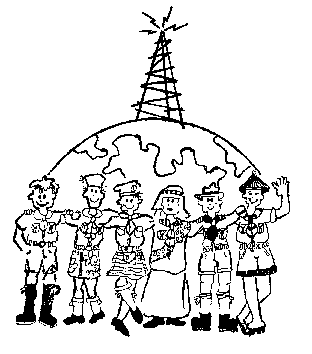
\includegraphics[width=3cm]{grafiki/bts.png}
  \end{center}
\end{wrapfigure}Najważniejszym ich osiągnięciem było stworzenie własnego systemu stopni i sprawności. Drugim ważnym ruchem był Ruch Przyszłość Harcerstwa, którego uczestnicy aktywnie pełnili różne funkcje i zadania w ZHP. Zasięg oddziaływania ruchu rozszerzały publikacje zamieszczane w Na Przełaj. Oba ruchy znacząco wpłynęły na postanowienia podjęte przez VII Zjazd. Podczas stanu wojennego działalność ZHP nie została zawieszona (choć zawieszono wtedy większość związków i stowarzyszeń). Na porządku dziennym znalazła się walka o udział umundurowanych harcerzy w uroczystościach religijnych. Droga do efektywnej pracy harcerskiej była otwarta, choć aparat etatowy był instytucją jedną z najbardziej odpornych na zmiany. Władze Związku wciąż patrzyły na władze państwowe i stosując zachowawczą politykę, bały się wykonać śmiałe kroki prowadzące do głębokich zmian.

Dopiero okrągły stół w roku 1989 i nastanie nowego porządku w Polsce spowodowały prawdziwe, będące powrotem do tradycji, zmiany w Związku dokonane po części na IX (XXVI wg. przywróconej na nim numeracji przedwojennej) Zjeździe w 1989 roku. Przywrócono przedwojenne Prawo i Przyrzeczenie. Ilość harcerzy od lat 80. (1980 - ponad 3 mln.) systematycznie maleje (dziś ok. 400.000). Jednak ta tendencja nie jest obecnie bardzo dynamiczna. W 1989 roku z półkonspiracyjnego, działającego w łonie ZHP, Ruchu Harcerstwa Rzeczypospolitej i Białej Służby (powstałej w 1982 roku na okoliczność II pielgrzymki Jana Pawła II do Polski) powstał Związek Harcerstwa Rzeczypospolitej, organizacja odwołująca się do zasad etyki chrześcijańskiej i tradycji narodowej, uważająca się za kontynuację przedwojennego ZHP (Stanisław Broniewski Orsza uważa się za jej ideowego twórcę, , a także inne organizacje harcerskie (z różnego rodzaju niezależnych ruchów): Związek Harcerstwa Polskiego 1918 (połączył się z ZHR w 1993 roku), Polska Organizacja Harcerska (obecnie połączona z ZHRem), Stowarzyszenie Harcerstwa Katolickiego Zawisza. Z lat biurokracji i centralnego sterowania pozostał zły społeczny obraz harcerstwa oraz zapaść harcerstwa starszego. W 1995 roku w wyniku uchwalenia przez Zjazd ZHP decyzji o zniesieniu wersji Przyrzeczenia Harcerskiego, w której nie składa się ślubu służby Bogu, od Związku odłączył się hufiec Warszawa-Śródmieście i utworzył Stowarzyszenie Harcerskie.
\chapter{System zastępowy}
\section{Wstęp}
\begin{wrapfigure}{l}{4cm}
  \begin{center}
    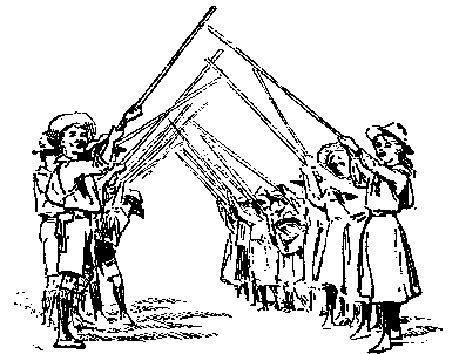
\includegraphics[width=4cm]{grafiki/szpaler.png}
  \end{center}
\end{wrapfigure}Kiedy  spojrzy się na  drużynę, od  razu rzuca  się w  oczy,  że nie jest ona jednolitą całością. 
W każdej grupie liczącej kilkanaście - kilkadziesiąt osób tworzą się  mniejsze  grupki (tak jak np. w  klasie). 
Stworzenie systemu zastępowego, przez Rolanda E. Philipsa było wyjściem na przeciw tworzeniu  się w drużynach właśnie takich małych grupek harcerzy, którzy wybierali sobie jednego spośród nich na przywódcę - zastępowego. 
Chłopcy zawierają  przyjaźnie  ze względu na: wiek, zainteresowania,  miejsce  zamieszkania, chodzenie do jednej klasy. Spełnienie trzech z tych kryteriów może być dobrym kluczem  do stworzenia  solidnego zastępu. 
	
Przy tworzeniu systemu zastępowego w drużynie nie należy nic narzucać, zastępy wytworzą się same, chłopacy sami dobiorą się w grupy, które potem staną  się zastępami. Sztucznie stworzony zastęp nie przejdzie próby czasu (długo się nie utrzyma, a ponadto, ma niewielkie szanse by skutecznie działać).

Gdy w danej grupie (przyszłym  zastępie)  znajduje  się  taki chłopak, który  zawsze ma najwięcej do powiedzenia  i  w  dodatku  pozostali  go  słuchają, wówczas z wyborem zastępowego nie ma problemu. 
Zastępowy powinien dbać o swoich harcerzy z zastępu,  a o rozwój zastępowych dbać powinien drużynowy poprzez prowadzenie zastępu zastępowych (w którym zastępowym jest drużynowy).

Praca zastępu zastępowych  nie powinna znacząco różnić się od pracy poszczególnych zastępów  w  drużynie. Dla wielu zastępowych zbiórki zastępu zastępowych, pod wodzą  drużynowego, mogą być swoistym poligonem doświadczalnym przed zbiórkami  poszczególnych zastępów. Zbiórka zastępu zastępowych na  oczątku tygodnia da możliwość zastępowym powtórzenia jej w  pozostałych dniach już ze  swoimi  zastępami.

System zastępowy nie oznacza tylko, że w drużynie istnieją zastępy, ale że drużynowy prowadzi drużynę przez zastęp zastępowych.

\begin{aquote}{Roland E. Philips}
  System  zastępowy  nie  jest  jedną  z  wielu  metod organizowania  pracy  skautowej, lecz jest  on  jedyną  metodą.
 \end{aquote}
 
 
\section{Zastęp}
\begin{wrapfigure}{l}{3cm}
  \begin{center}
    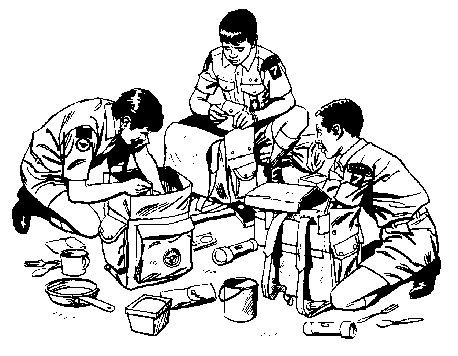
\includegraphics[width=3cm]{grafiki/zastep.png}
  \end{center}
\end{wrapfigure}No, a co to jest ten zastęp? - zastęp jest to grupa chłopców w mniej więcej jednakowym wieku, o tych samych zainteresowaniach i pochodzących z  tego samego środowiska (szkoła - klasa, osiedle - podwórko). 
Liczba  chłopców  w  zastępie  powinna  być około 6 - 8. Pozwala to na dobrą pracę zastępu i oddziaływanie zastępowego  na swoich harcerzy (stopnie, sprawności, zabawa, wykonywanie różnych zadań, wspólne życie obozowe). 
Na czele zastępu stoi zastępowy. 
Jest to chłopiec  o najmniej w tym samym  wieku co członkowie zastępu. Wybija się on spośród nich dzięki swoim zdolnościom przewodzenia w grupie. 
Powinien być wybierany przez zastęp. 
Zastępy mogą być jednopoziomowe, gdy są nim chłopcy w jednym wieku, z jednej akcji naborowej lub wielopoziomowe, gdy co roku, ktoś z zastępu przechodzi do drużyny wędrowniczej, a na jego miejsce dochodzi ktoś nowy.

Pamiętajmy,  że zastęp jest najistotniejszą jednostką naszej organizacji. 
To od zastępu zależy poziom drużyny. 
Każdy zastępowy powinien wiedzieć, że w zastępie wyłaniają się nowe jednostki mogące dalej pozytywnie wpływać  na  rozwój  drużyny.

Silne zastępy to silna organizacja, a silna organizacja to miejsce kształtowania obywateli do  służby dla naszej Ojczyzny.
	
\section{Zastępowy}
Czas teraz zastanowić się, kto to właściwie jest zastępowy. Kim Ty masz być? Zastępowy to ktoś szczególny. To harcerz, który obok drużynowego ma do zrobienia najwięcej w drużynie. Jest to służba, trudna służba, która jednak dobrze wykonywana jest bardzo owocna. \begin{wrapfigure}{r}{4cm}
  \begin{center}
    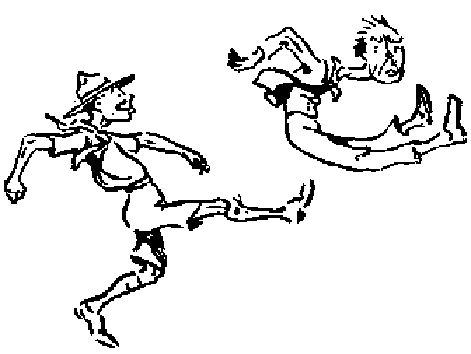
\includegraphics[width=4cm]{grafiki/kop.png}
  \end{center}
\end{wrapfigure} 
	Zastępowy jest jeden a chłopaków wielu. To nieprawda. Zastępowych jest trzech, a wszystko to w jednej osobie.
\begin{itemize}
\item \textbf{Pierwszy zastępowy  to  wzór.}
\item \textbf{Drugi zastępowy to wódz.}
\item \textbf{Trzeci jest  starszym bratem.}
\end{itemize}


Trzy twarze jednego, bardzo ważnego człowieka. Jest wzorem, bo taki, jaki będzie on, tacy będą jego harcerze z zastępu. Wódz - znaczy przewodnik, facet, który ma wśród chłopaków siłę przebicia, słowem odpowiedzialny młody człowiek. Jeżeli zastępowy będzie kumplem, pomocnikiem, opiekunem to będzie starszym bratem. Dzięki tym trzem twarzom zastępowy może samodzielnie prowadzić zastęp i mieć tak wielki wpływ na chłopaków, że może zrobić z nich morowych chłopaków.
	Dobry  wódz musi pamiętać o tym, że niezbędna jest praca ze wszystkimi  harcerzami  ze  swojego  zastępu. Tylko dzięki takiej pracy będą najlepsi.  Tylko wówczas, gdy będą razem zdobędą szczyty.
	Zastępowy koniecznie chce być w swojej pracy najlepszy. Tu objawia się zastępowy - wzór. Musi pokazać swojemu zastępowi, że potrafi  słuchać i wykonywać rozkazy bez względu na to, czy jest obecny  drużynowy czy nie. Nieodzowne jest przodowanie zastępowego w zdobywaniu stopni i sprawności. Zastępowy - wzór sprawdza się w każdych warunkach i dlatego chłopcy pójdą za nim bez zbędnych tłumaczeń.

Nie można jednak zapomnieć, że (jak pisał Robert Baden - Powell): musicie nimi kierować a nie popychać ich. 

\noindent
Pamiętajcie także, że zastępowy:
\begin{itemize}\itemsep1pt

\item znawca technik harcerskich
\item  świeci przykładem: styl harcerski, pogoda ducha, nauka, dom, kultura, pomoc bliźnim
\item  dba o wszystko w  zastępie:  począwszy od  tego czy jego harcerze noszą pas  w szlufkach, przez tworzenie nowych gier, wyjazdy na wycieczki, czy biwaki, aż do zdobywania sprzętu na obozy.
\item  prowadzi zastęp wg planu, który wymyślił wraz zastępem - pisze więc mądry plan działania i konsekwentnie go realizuje, aż osiągnie cel. Prowadzi też książkę lub zeszyt zastępowego (nie na  pokaz  tylko dla samego  siebie), gdzie ma listę swoich harcerzy, notatki o nich, sieć alarmową, plan działania, plany zbiórek, comiesięczny rachunek sumienia (co się udało a co nie), decyzje Rady Zastępu i Rady Drużyny i wszystko co jeszcze jest mu potrzebne w pracy zastępu.
\item  zna i wciąż poznaje: problemy, zdolności, zainteresowania, niepowodzenia itp. swoich harcerzy z zastępu.
\item   widzi, że każdy chłopiec z zastępu jest inny: zastęp to nie szara masa identycznych chłopaków, jeśli to zacznie dostrzegać to będzie wiedział,  że  z każdym chłopakiem trzeba pracować osobno.
\item  uczy chłopaków odpowiedzialności za siebie i  innych.
\item  nie jest dla harcerzy kapralem i ograniczeniem, lecz pociąga ich za sobą.
\end{itemize}

I jeszcze jedno:
\begin{aquote}{Hm. P. Stawiński HR}
Zastępowy  nosi  głowę  w chmurach, ale  nogami  mocno  stąpa  po  ziemi.
 \end{aquote}



\section{Duchowość zastępowego}

Zastanawiasz się czasem, czy harcerz to ktoś wierzący w Boga? – tak, to ktoś właśnie taki. Co więcej, harcerz to wzór życia duchowego, moralności – sami wiecie jak często jest z tym u nas trudno. Tym większa rola zastępowego.

W wielu domach rodzice nie przekazują już wiary, nie jest ona silna. Ty masz za zadanie być wówczas kimś, kto kieruje także duchowości swojego zastępu. Twój zastęp, to taki mały Kościół, który został przez Boga powierzony właśnie Tobie. Powinieneś dbać o to, czy chłopcy chodzą do Kościoła, do spowiedzi, czy się modlą, robią rachunek sumienia, czy starają się być lepsi każdego dnia. Wiadomo, nie można ich do tego zmuszać, ale zachęcać. \begin{wrapfigure}{r}{3cm}
  \begin{center}
    
\includegraphics[width=3cm]{grafiki/duchowosc.png}
  \end{center}
\end{wrapfigure} W jaki sposób? – proste, przykładem własnym. Kiedy Ty będziesz się modlił, uczestniczył we Mszy św., kiedy będziesz lektorem i będziesz dobrym człowiekiem, oni bardzo szybko zapragną być tacy jak Ty. Wówczas szybko staną obok Ciebie przy ołtarzu, czy w kolejce do konfesjonału. Widzisz jakie to proste. Proszę też, abyś czasem modlił się za swoich chłopców w zastępie, drużynowego, to także wielka dla nich pomoc. Nie zapomnij też, ze masz obok kapelana, który może Ci zawsze pomóc.

Na obozie zaś nie zapominaj o modlitwie porannej, wieczornej, przed posiłkami, po nich, o Mszy św., o wieczornym rachunku sumienia i o tym, że Bóg jest gdzieś blisko, może nawet w drugim człowieku\ldots
\chapter{Działania zastępu}

\section{Plan pracy zastępu}

Napisanie planu pracy zastępu, to połowa sukcesu. Jeśli będziesz według niego działał, to wówczas możesz być pewny, ze żadna twoja zbiórka nie będzie nudna, a zastęp będzie ciągle się powiększał. Plan pracy składa się z:
\begin{itemize}[noitemsep] 
\item \textbf{Strony tytułowej}
\item \textbf{Ogólnej charakterystyki zastępu} --- opis sytuacji, cele długofalowe, cele na rok pracy materialne;
\item \textbf{Szczegółowej charakterystyki zastępu} --- tu zamieszczamy opis każdego przedstawiciela zastępu: wiek, szkołę, ilość lat w harcerstwie, przebieg jego służby, pasje i to, nad czym powinien popracować; charakterystyka powinna być dość szczegółowa, gdyż przecież znasz swój cały zastęp;
\item \textbf{Cele szczegółowe na rok pracy}
\item \textbf{Szczegółowy plan pracy} --- nie zapomnij, że zbiórki zastępu masz co tydzień, a raz w miesiącu zbiórkę drużyny; tu opisujesz planowany temat zbiórki i ogólnie zajęcia, jakie przeprowadzisz na niej.
\end{itemize}

\noindent
Co najważniejsze, plan powinieneś oddać do 03 IX każdego roku, aby drużynowy na podstawie planów pracy wszystkich zastępów, stworzył plan pracy drużyny. 

\section{Obrzędowść zastępu}
Każdy naród posiada swój język i własną kulturę. Właśnie to wyróżnia go spośród innych. \begin{wrapfigure}{r}{3cm}
  \begin{center}
    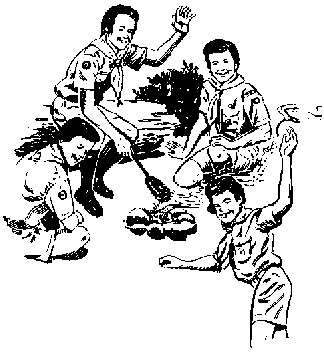
\includegraphics[width=3cm]{grafiki/happy.png}
  \end{center}
\end{wrapfigure} Podobnie jest i w  harcerstwie. Mimo, że wszystkim nam  chodzi o to samo, coś sprawia że harcerze z 15 PDH, różnią się od tych z 1 ŁDH. To  coś  to  nie  tylko  barwy i numer, ale wszystko to, co jest językiem i kulturą drużyny - obrzędy.
	Po co komu obrzędy? Jest  kilka  odpowiedzi:
\begin{itemize}[noitemsep,nolistsep] 
\item  tradycja --- ludzie się zmieniają,  świat się zmieni,  ale obyczaje zostaną;
\item  język --- którym mówi się chłopakom o co tu  właściwie chodzi;
\item  dyscyplina --- ułatwia techniczne prowadzenie np. zbiórki czy ogniska;
\item  jedność --- my mamy swoje obrzędy;
\item  przyciąganie ---  tajemnica intryguje;
\item  i wiele innych rzeczy.
\end{itemize}
	Czy tylko drużyna może posiadać obrzędowość? Nie, oczywiście także zastępy muszą mieć swoje obyczaje. Ale:
	\begin{itemize}[noitemsep,nolistsep] 
\item  muszą one współgrać z obyczajami drużyny
\item  nie może być  ich zbyt  dużo  aby  nie  przytłaczały
\item  muszą być nijako przy  okazji - chłopacy nie mogą całą zbiórkę wkuwać obrzędów
\item  nie wolno ich zmieniać bez powodu.
\end{itemize}
\begin{wrapfigure}{l}{4cm}
\begin{center}
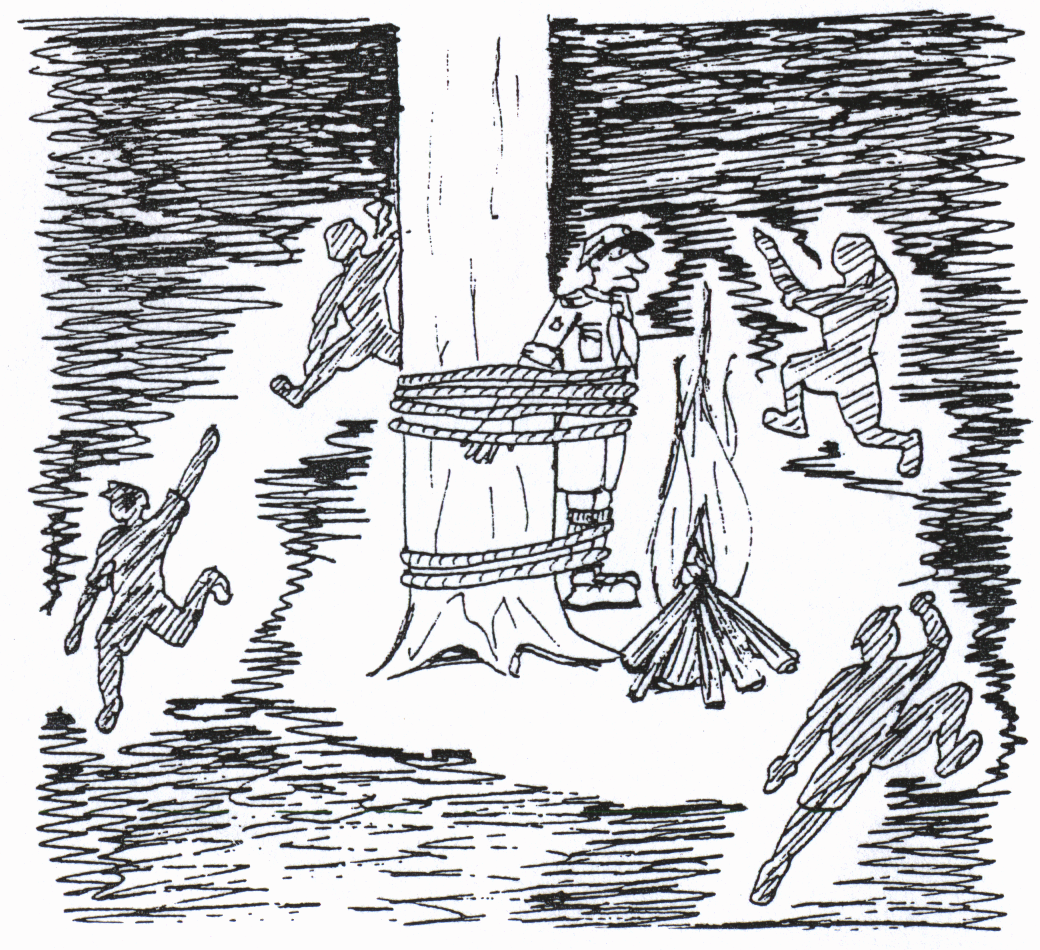
\includegraphics[width=4cm]{grafiki/drzewo.png}
\end{center}
\end{wrapfigure}Obrzędy i obyczaje  mogą  być  bardzo  różne:  od  sposobu  noszenia  proporca, przez  jakiś  znak  zastępu,  do  koloru  sznurowadeł  funkcyjnych zastępu  włącznie.  Ale uwaga! Obrzędowość nie  może być zbędnym balastem - musi pomagać, a nie  przeszkadzać.

Kiedy chcesz stworzyć nowy obrzęd,  zastanów się po co chcesz to  zrobić. 
 
\clearpage	
\section{Zbiórka zastępu}

Pytasz sam siebie: po co nam właściwie te zbiórki? 
Niezbyt kulturalnie można by odpowiedzieć pytaniem: a po co Wam właściwie harcerstwo?

Po to, żeby co dzień być trochę lepszym, trochę więcej umieć, trochę więcej wiedzieć, żeby  w końcu spędzić  sensownie czas, a to wszystko w kontekście celu wychowawczego ZHRu, o którym mówiliśmy już wcześniej.
	
No więc zostawił Cię Twój  okrutny drużynowy z zadaniem  przygotowania  zbiórki. 
Im bliżej terminu tym bardziej się denerwujesz. 
A może by tak nie pójść? 
Udać chorego? 
Eee\ldots

\begin{figure}[h]
\begin{center}
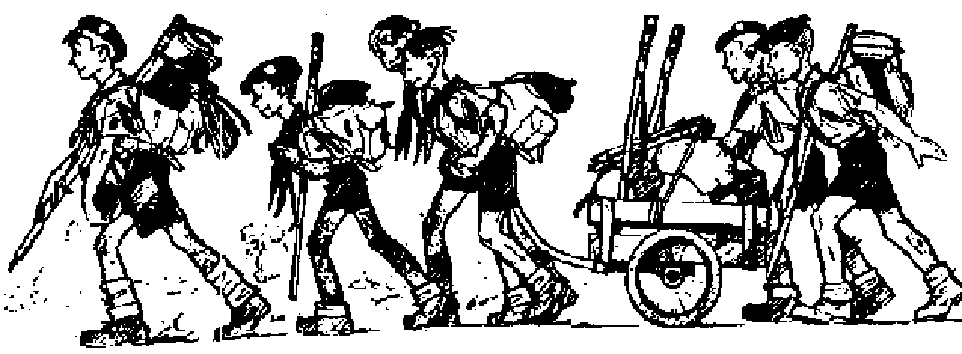
\includegraphics[width=0.9\textwidth]{grafiki/zbiorka.png}
\end{center}
\end{figure}
	
Siadasz w końcu nad kartką i rozmyślasz co by tu zrobić. Coś tam piszesz i  idziesz na zbiórkę. 
	
A może użyć  na  początek  takiego schematu:

Po co, czyli jaki \textbf{SENS} ma ta zbiórka? 
(kiedy chłopacy wrócą ze zbiórki muszą jednym zdaniem powiedzieć co robili: pełnili służbę w domu dziecka, grali w piłkę, zdobywali sprawności, odwiedzali super człowieka, harcowali po lesie) 
Pamiętaj, że oni zaraz wyczują, że zbiórka jest  tylko posklejana bez ładu z różnych gier.

Musi być \textbf{POMYSŁ}. czasem szalony, nierealny, ale porywający. Zrobić grę w niedostępnej części muzeum, odwiedzić drużynowych Twojej drużyny z ostatnich dziesięciu lat, zaprosić komandosa, urządzić bieg na podstawie aktualnego filmu z Jamesem Bondem, wleźć na czubek ratusza\ldots

Żeby to przeprowadzić musi być \textbf{PLAN}, czyli jak wprowadzić w życie mój (nasz) pomysł.
Gra  wg filmu Na  krawędzi z Sylwestrem Stallone:
\begin{enumerate}[noitemsep,nolistsep] 
\item spotkanie na Cytadeli;
\item szukanie walizki z milionem dolarów wg planu rozdanego wcześniej;
\item pokonanie przeciwników podczas podejścia pod najwyższą możliwą górę (a jak  się  ich  pokonuje?);
\item odnalezienie walizki z \ldots czekoladą w środku.
\end{enumerate}
A jaki był  sens tej zbiórki? 
O choćby ćwiczenia fizyczne podczas gonitwy, nauka czytania planu, podchodzenia, uczciwa walka itd.
	
Dużo czasu  zajmuje \textbf{PRZYGOTOWANIE} , ale nie zawsze sam musisz  rysować plan, przynosić walizkę i czekoladę, tasiemki do zrywania w pojedynkach. 
Rozdziel zadania.

Wróciłeś ze zbiórki. Podobało  się chłopakom?
Zapytaj siebie, czy gdybyś jej nie  przygotował, ale uczestniczył w takiej zbiórce przyszedłbyś na następną?
	
Może zapomniałeś o \textbf{ATMOSFERZE}? 
Ona nie zależy od terenu, miejsca. 
Ona zależy  od Ciebie! 
Traktowałeś wszystkich równo? 
Nie darłeś się na harcerzy? 
Opowiedziałeś kawał? 
To właśnie powoduje, że zbiórka nie jest lekcją!!!
\begin{wrapfigure}{l}{3cm}
\begin{center}
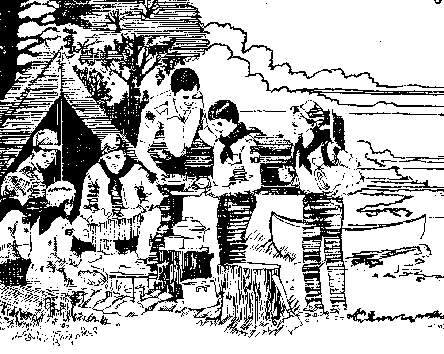
\includegraphics[width=3cm]{grafiki/zbiorkazastepu.png}
\end{center}
\end{wrapfigure}
\section{Zasady dobrej (Twojej) zbiórki}

Kiedy już opracujesz plan swojej zbiórki możesz sprawdzić czy zachowane są poniższe zasady. Nie przygotowuj zbiórki patrząc na tę ściągę. Czasem trzeba z któreś zasady zrezygnować na rzecz innej. Oceń swój plan i już  przeprowadzoną zbiórkę z tą listą. Wkrótce Twoje plany same się z nią zgodzą - nie będziesz już potrzebował ściąg.
\begin{description}


\item
[ZASADA 1 ZBIÓRKA MA LOGICZNY  CIĄG]
Jeden element zbiórki wypływa z drugiego. 
Z gawędy gra. 
Z gry - nauka  technik. 
Z technik - znów gra. 
Z gry - piosenka i tak dalej. 
Jeśli o tym zapomnisz, to ciągle będziesz zerkał do kartki z przygotowaną zbiórką (lekcje?),  a chłopcy zawsze to wyczują. 
Oni nie lubią drętwych zbiórek.
\item 
[ZASADA 2 CHARAKTER ZAJĘĆ MUSI  SIĘ ZMIENIAĆ]
Kiedy planujesz zbiórkę pamiętaj, że zbyt jednolite zajęcia nużą. 
Szybciej  spokojne, ale ruchowe także. 
Więc tak pozmieniaj kolejność zajęć  żeby mieszały się powaga (gawęda) z wesołością (piosenka), cisza (kominek) z hałasem (okrzyk  zastępu) spokój (praca rąk) z ruchem (gra ruchowa, turniej) dyscyplina (musztra, apel)  z luzem (zwiad,  gra).
\item
[ZASADA 3 ZBIÓRKA MUSI MIEĆ TEMPO]
Zanim ktokolwiek zapyta: czemu ta przerwa?, Ty musisz już przedstawić następny punkt programu. W czasie prowadzenia  gry,  mówienia gawędy i ćwiczenia węzłów, patrz czy  chłopcy się nie kręcą, nie zaczynają opowiadać kawałów. 
Wtedy  przerwij nawet jeśli nie zrobiłeś wszystkiego. 
Kończ  zbiórkę zanim się znudzą, wtedy chętniej przyjdą na następną.
\item
[ZASADA  4 ZASTĘPOWY JEST Z NAMI]
Nie siedź  z boku przyglądając się harcerzom. 
Weź udział w grze, najgłośniej się wydzieraj w okrzyku zastępu. 
Nie baw się w dyrektora, bądź jednym  z nich.
\item
[ZASADA  5 ZBIÓRKA  MA  CZTERY  STAŁE  ELEMENTY]
Obrzęd powitania, gawęda - to może być  wizyta fajnej osoby, dyskusja lub ciekawie opowiedziana historia - 5 minut to dosyć, nigdy nie przekraczaj 10 minut (5 minut gawędy to 20 minut jej przygotowywania w domu!), Rada Zastępu - tu  przekażesz sprawy bieżące,  tu  rozwiążecie wspólny problem, pomyśl nad obrzędem rozpoczęcia (może np. postawicie między Wami proporzec zastępu?), niech Rada trwa nie dłużej niż 15 minut, obrzęd pożegnania -  może jakiś specjalny Wasz krąg, krótka piosenka, może coś jeszcze innego?
\item
[ZASADA  6 COŚ NOWEGO I COŚ STAREGO NA KAŻDEJ ZBIÓRCE]
To chyba jasne? 
Przez przypomnienie znanych rzeczy, łączysz zbiórkę z poprzednią, wprowadzasz klimat. 
Możesz też utrwalić, przypomnieć to, co łatwo  się  zapomina.
\item
[ZASADA 7 NIE MA ZBIÓRKI BEZ INICJATYWY CHŁOPAKÓW]
Ciesz się kiedy chłopcy mają własne pomysły, chcą nagle przypomnieć starą grę, ulubioną piosenkę, zmienić przeprowadzaną przez Ciebie zabawę. 
To znaczy, że traktują zbiórkę jak swoją, chcą żeby była jak najfajniejsza. 
Nie możesz ich wiecznie pouczać, dyrygować  nimi. 
Jeśli w czasie zbiórki zdarzy się coś niezwykłego nie trzymaj się kurczowo napisanego  planu, ale wykorzystaj okazję żeby coś nowego poznać, zobaczyć, a zwłaszcza zrobić dobry  uczynek.
\item
[ZASADA  8 ZAWSZE DZIELIMY PRACĘ]
Jeśli zawsze sam przygotowujesz zbiórkę, to w końcu wyczerpią Ci się pomysły. Poza tym nauczysz harcerzy czekania na to, co będzie zamiast współtworzenia zbiórek.

Daj im zadania: przynieść tekst piosenki, życia do gry w terenie, busolę itd. Jeśli trzeba zaprosić gościa niech załatwią to chłopacy. Tylko pamiętaj: jeśli przed zbiórką nie zadzwonisz z pytaniem o wykonanie zadań, możesz się znaleźć w sytuacji, w której zabraknie Ci głównego punktu zbiórki!
\item
[ZASADA  9 NIESPODZIANKĘ ZAWSZE SIĘ WSPOMINA]
Staraj się przynajmniej co jakiś czas zaskoczyć mile chłopaków. Nie daj  im  pomyśleć,  że  wpadasz  w  rutynę i przyzwyczajenia.
	
	Co to może być? Musisz już sam wymyślić: ciekawą osobę, film video,  zbiórkę z zastępem harcerek...
\end{description}
	Że co? Że niby dużo tej teorii? Jeśli parę razy przygotujesz zbiórkę według  tych  paru zasad, same Ci  wejdą w krew i nawet nie będziesz wiedział kiedy i jak. Ale nie zaszkodzi  o jakiś czas tu zerknąć i  sobie  przypomnieć.
\begin{itemize}

\item ZASADA 1 - LOGICZNEGO  CIĄGU
\item ZASADA 2 - PRZEMIENNOŚCI ELEMENTÓW ZBIÓRKI
\item ZASADA 3 - TEMPA
\item ZASADA 4 - ZASTĘPOWY TEŻ JEST Z NAMI
\item ZASADA 5 -  CZTERECH  STAŁYCH  ELEMENTÓW ZBIÓRKI
\item ZASADA 6 -  COŚ  STAREGO I  COŚ NOWEGO NA ZBIÓRCE
\item ZASADA 7 -  SAMODZIELNOŚCI I INICJATYWY CHŁOPCÓW
\item ZASADA 8 - PODZIAŁU PRACY
\item ZASADA 9 - POZYTYWNEGO ZASKOCZENIA I NIESPODZIANKI

\end{itemize}
Na koniec coś co może Tobie  ułatwić planowanie zbiórek. To formy pracy:

Formy podstawowe:
-  ognisko	-  gawęda	- pląs 		- ćwiczenie
- okrzyk 	-  pokaz		- kominek	- zwiad
-  śpiewy	-  zadanie	- popis		- quiz
-  szkolenie	-  bieg		- turniej		- dyskusja
- rozmowa	-  obrzędy	- festiwal	- zawody
-  apel		-  musztra	- praca rąk	- próba
- gra		- harc		- alarm		-  podchody
- konkurs	- herbatka	- służba
- zadania zespołowe		- zadania międzyzbiórkowe
- działania społeczne			

Formy złożone :
-  zbiórka	-  obóz		-  biwak		-  włóczęga
-  zlot		-  kolonia	-  wycieczka	-  zimowisko
-  rajd		-  złaz


\section{Konflikty i problemy w zastępie}



\begin{wrapfigure}{l}{3cm}
\begin{center}
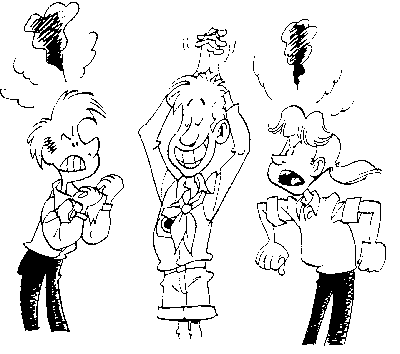
\includegraphics[width=3cm]{grafiki/konflikty.png}
\end{center}
\end{wrapfigure}\begin{aquote}{Ernst Bloch}
Rekin i słoń nie mogą się spotkać i nie stoczą ze sobą walki. Ale już wszystko, co żyje w tej samej wodzie, czy chce czy nie chce, tworzy jedność, w której możliwa jest i wojna i porozumienie
 \end{aquote}


Nie  wszystko  zawsze w  zastępie  funkcjonuje idealnie. 
Zresztą  dobrze  jest  gdy  w  zastępie  zdarzają się od czasu do  czasu burze,  byle tylko  dobrze  się kończyły.  Problemów, które  zwykle  jak  grom z  jasnego nieba spadają na zastępowego może być bardzo wiele. Jeden z chłopców często opuszcza  zbiórki, dwóch innych chce zmienić  zastęp,  a w ogóle to wszyscy o byle co  się kłócą itp.
	Jak z tym sobie radzić?  Sposobów jest bardzo wiele, często wybiera się ucieczkę, ignorowanie (niezauważanie problemu lub celowe jego pomijanie) jako metodę rozwiązania konfliktu, że nie są  to idealne  sposoby  zaradzania  problemom, nie trzeba chyba  specjalnie  przekonywać bo ucieczka czy ignorowanie zwykle kończy się rozbiciem zastępu lub bezsensowną rezygnacją zastępowego z pełnionej funkcji. Przecież Ty jesteś zastępowym bo umiesz sobie radzić z konfliktami  i  problemami lepiej niż inni. to garść dobrych rad, które powinny pomóc Wam rozwiązywać  konflikty, nie tylko te w zastępie ale także w  życiu.

1.
Trzeba zdać sobie sprawę, że problemy i konflikty zarówno w  życiu jak i w zastępie są nieuniknione.

2.
Problem trzeba zauważyć, a więc trzeba mieć oczy i uszy otwarte.

3.
Zadaj sobie pytanie: dlaczego? Jaka jest przyczyna problemu, konfliktu.

4.
Szukaj prawdziwej odpowiedzi na powyższe pytania, nie daj  się zwieść temu co mówią inni, lub czym Tobie oczy  mydlą  strony konfliktu. Czasem potrzeba Twardej konfrontacji poglądów z zainteresowanymi stronami konfliktu.
5.
Rozwiązanie konfliktu spróbuj znaleźć sam, gdy będziesz wiedział  gdzie naprawdę tkwi problem nie powinno to być trudne, jeśli nie możesz sobie poradzić sam, jest zawsze  gotowy Twój  starszy brat - drużynowy.

6.
Ostateczne rozwiązanie problemu dobrze jest przegadać z drużynowym. Czasem wręcz konieczna jest interwencja drużynowego  w  problem, szczególnie gdy do konfliktu dochodzi między Tobą – zastępowym, a którymś z  chłopaków.


Pamiętajcie, że wyrzucenie kogoś z zastępu z powodu jakiś niejasnych nieporozumień, czy konfliktów to jest nasza porażka. Spróbujmy teraz prześledzić wg  powyższego  wzoru jeden prosty konflikt. Jeden z harcerzy - niech będzie Jasio, nagle przestał przychodzić na zbiórki zastępu. Niby nic, ale w pewnym momencie drużynowy zaczyna zastępowemu wiercić dziurę w brzuchu w  sprawie Jasia.

1.
Warunek  pierwszy  został   spełniony,  mamy  problem.

2.
Być  może  zastępowy  sam zauważył problem ale na niego nie  zareagował, więc drużynowy pokazał go zastępowemu. 

3.
Teraz zastępowy sam musi się zastanowić:  dlaczego Jasio nie  przychodzi na zbiórki? Może dlatego,  że ma problemy w  szkole,  może  jest chory, może któryś z chłopaków bardzo mu na zbiórkach dokucza,  może... Każdy problem trzeba przeanalizować. Zastępowy myślał i nagle spojrzał do  swojego notatnika zastępowego i zobaczył, że jeszcze dwa miesiące  temu na  zbiórki przychodził cały zastęp - 8 osób,  a teraz  na  zbiórkach bywa 4 - 5 chłopców, czyli inni też  opuszczają  zbiórki,  może  tylko nie tak często jak nasz Jasio. Więc może zbiórki są mało  ciekawe,  chłopcy  się na nich dobrze nie czują...

4.
Swoją teorię powinien zastępowy sprawdzić  w rozmowie z chłopakami, a szczególnie z Jasiem. Okazało się, że miał  rację,  zbiórki  stały się mniej atrakcyjne, a ponadto Jasio ma problemy w szkole  z matmy.

5.
Zastępowy poznał problem,  teraz trzeba go tylko rozwiązać. Zbiórki powinny stać się bardziej  atrakcyjne. Odpowiedź na pytanie, jak to  robić,  znalazłeś w innej  części tego notatnika. Może warto każdą zbiórkę przygotowywać wspólnie z jednym z chłopaków,  za każdym razem  z innym? Co do problemów Jasia z matmą, przecież jego zastępowy ma 6 z matmy co za problem dać mu dwa razy  w tygodniu korki,  poprawi  oceny i  znów  może  przychodzić na  zbiórki.

6.
Rozwiązanie problemu gotowe, ale warto pogadać o tym z drużynowym. To drużynowy powinien porozmawiać  z rodzicami Jasia i zaproponować takie, czy inne rozwiązanie problemu.


\section{Nagrody i kary}
Między  karami i nagrodami musi być odpowiednia równowaga. Nie można tylko karać, tak jak samo nagradzanie nie rozwiąże wszystkich problemów. Pamiętajcie o tym, że fakt, iż musimy chłopaka z zastępu ukarać wynika często z naszego niedopatrzenia. Jeżeli chłopak robi coś źle, np. wycina swoje  inicjały w drzewie, to może nikt  mu nie  wytłumaczył, że  takie postępowanie nie przystoi harcerzowi.
\begin{wrapfigure}{l}{3cm}
\begin{center}
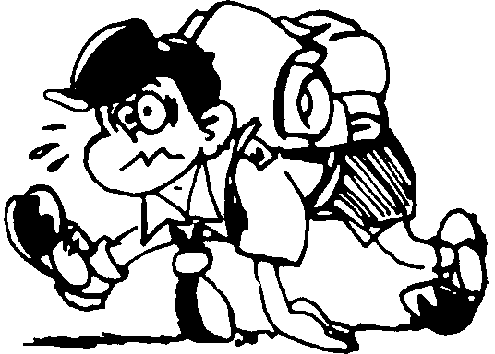
\includegraphics[width=3cm]{grafiki/plecak.png}
\end{center}
\end{wrapfigure}
Czasem, gdy chłopak coś przeskrobie wystarczy szczera męska rozmowa w cztery oczy. Gdy jednak to nie wystarcza może trzeba zwrócić uwagę chłopakowi przy pozostałych harcerzach zastępu  np. podczas wieczornego podsumowania dnia w zastępie. Czasem i ten sposób zawodzi albo przewinienie jest takie, że trzeba winnego  ukarać. Wówczas pamiętajcie, że każda kara musi mieć sens! Za każdym razem wytłumaczyć musicie dokładnie za  co  jest kara i na  czym  ma  ona polegać. Chciałbym Wam zaproponować dwa sposoby  karania.

Pierwszy to odsunięcie harcerza od pracy,  tzn. chodzi z zastępem wszędzie ale nie bierze udziału w tym co zastęp robi, a czas kary powinien wykorzystać na przemyślenie swojego błędu. 

Drugi sposób to dać możliwość naprawienia szkody którą wyrządził. Jeśli okaleczył drzewo, to niech pójdzie do leśniczego i jeden dzień przepracuje przy pielęgnacji szkółki leśnej, a wieczorem zda raport ze swojej pracy i przemyśleń nad złem które wyrządził. Jeśli zniszczył drugiemu prycz w namiocie niech ją podczas ciszy poobiedniej naprawi, a dodatkowo wykona jakiś element wyposażenia do namiotu zastępu. Niech kara którą wymierzacie uczy szacunku do pracy, przyrody i innych.

Pamiętajcie! Służba nie powinna być karą. Pełnić służbę to zaszczyt, choćby była trudna i niewdzięczna. Również nie mają większego sensu kary  w stylu biegania z plecakami, czy  robienia iluś tam pompek. Takie kary to ostateczność.

Nagrody. Nagradzaj każde dobre postępowanie harcerza. Niech by to była tylko ustna pochwała, ale przy  wszystkich członkach zastępu. Wytłumacz wówczas co takiego dobrego było w postępowaniu nagradzanego chłopaka. Dasz  innym wzór do naśladowania. Staraj się unikać nagród rzeczowych  w  stylu  np. ktoś przychodzi wzorowo umundurowany na zbiórkę to dostaje czekoladę. Doprowadzisz tylko do tego, że bez konkretnej nagrody chłopcy nic nie zrobią. Możesz np. chłopakowi, który przyszedł wzorowo umundurowany na zbiórkę pozwolić dokonać przeglądu mundurowego zastępu, w tym także Twojego  umundurowania.  a  pewno będzie  dumny, że mógł  sprawdzić   samego  zastępowego, a inni z pewnością będą mu nieco  zazdrościli.

Na koniec jedna ważna uwaga! Jeżeli chcecie ukarać lub nagrodzić kogoś zróbcie to jak najszybciej, a więc zaraz po zdarzeniu, wówczas chłopcy dokładnie wiedzą za co jest kara czy nagroda. Jeśli pochwalicie kogoś w czerwcu za to, że przyszedł na zbiórkę w lutym wzorowo umundurowany, to nikt nie będzie już  tego pamiętał, a z pewnością nikt nie będzie pamiętał jak był ten chłopak umundurowany, więc odpadnie możliwość naśladowania. Nagroda podobnie jak kara ma wychowywać, czyli mieć jakiś sens!

Zastanów się, jakbyś ukarał harcerza ze swojego zastępu, który ukradł na obozie  koledze czekoladę (i zjadł  ją sam), a jak ukarał byś harcerza, który podczas gry  oszukiwał i nie trzymał się wcześniej ustalonych zasad?

\begin{figure}[h]
\begin{center}
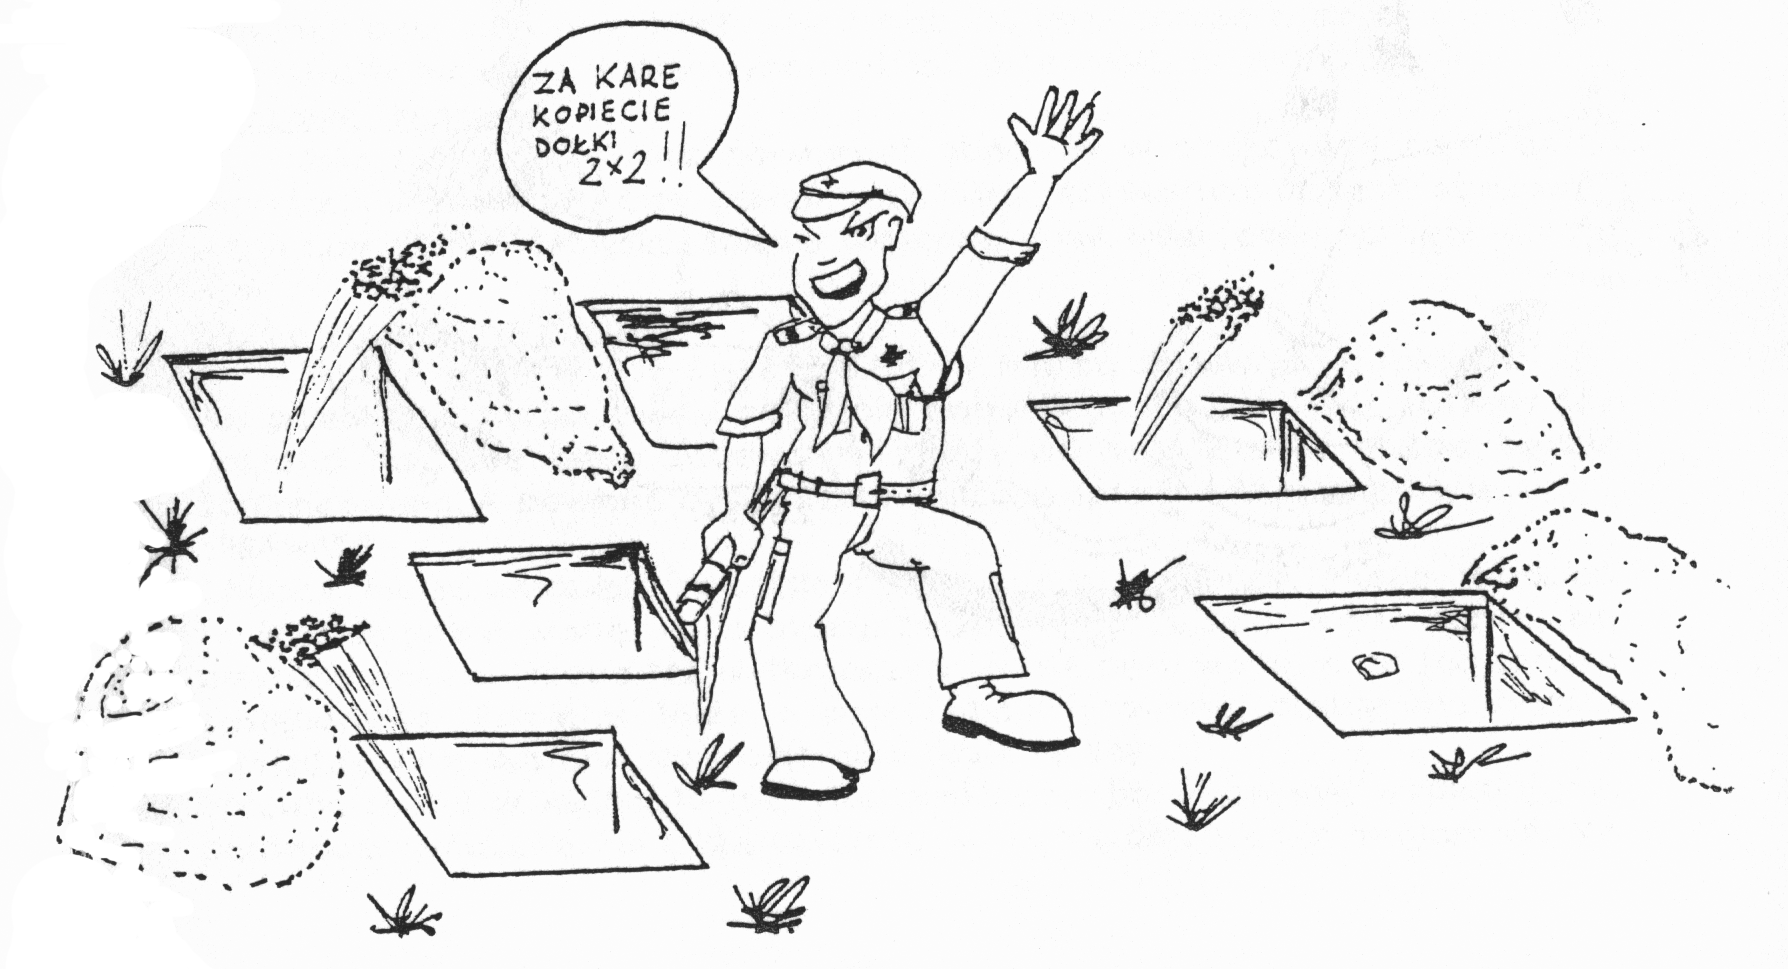
\includegraphics[width=0.8\textwidth]{grafiki/kara.png}
\end{center}
\end{figure}
	


\section{Sieć alarmowa zastępu}
\begin{wrapfigure}{l}{3cm}
\begin{center}
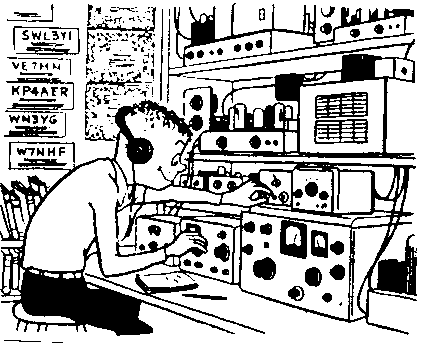
\includegraphics[width=3cm]{grafiki/nasluch.png}
\end{center}
\end{wrapfigure}Sieć alarmowa to sposób szybkiego przekazywania informacji pomiędzy kreślonymi osobami (członkami drużyny zastępu), przy użyciu najnowszych osiągnięć techniki (telefon, internet, łącza satelitarne, rower, samolot  itd.) oraz najstarszych darów natury (nogi, ręce, struny głosowe itd.). Bez łączności z tym, kto z nami wchodzi na szczyt, na pewno się tam nie dostaniemy. Sieć alarmową powinien posiadać każdy zastęp i drużyna, ponieważ bardzo ułatwia on pracę w drużynie oraz pozwala na zaoszczędzenie pieniędzy drużynowego lub zastępowego (na  telefony)  i czasu (potrzebnego na odwiedzenie i przekazanie informacji 150 harcerzom).

\begin{figure}[h]
\begin{center}
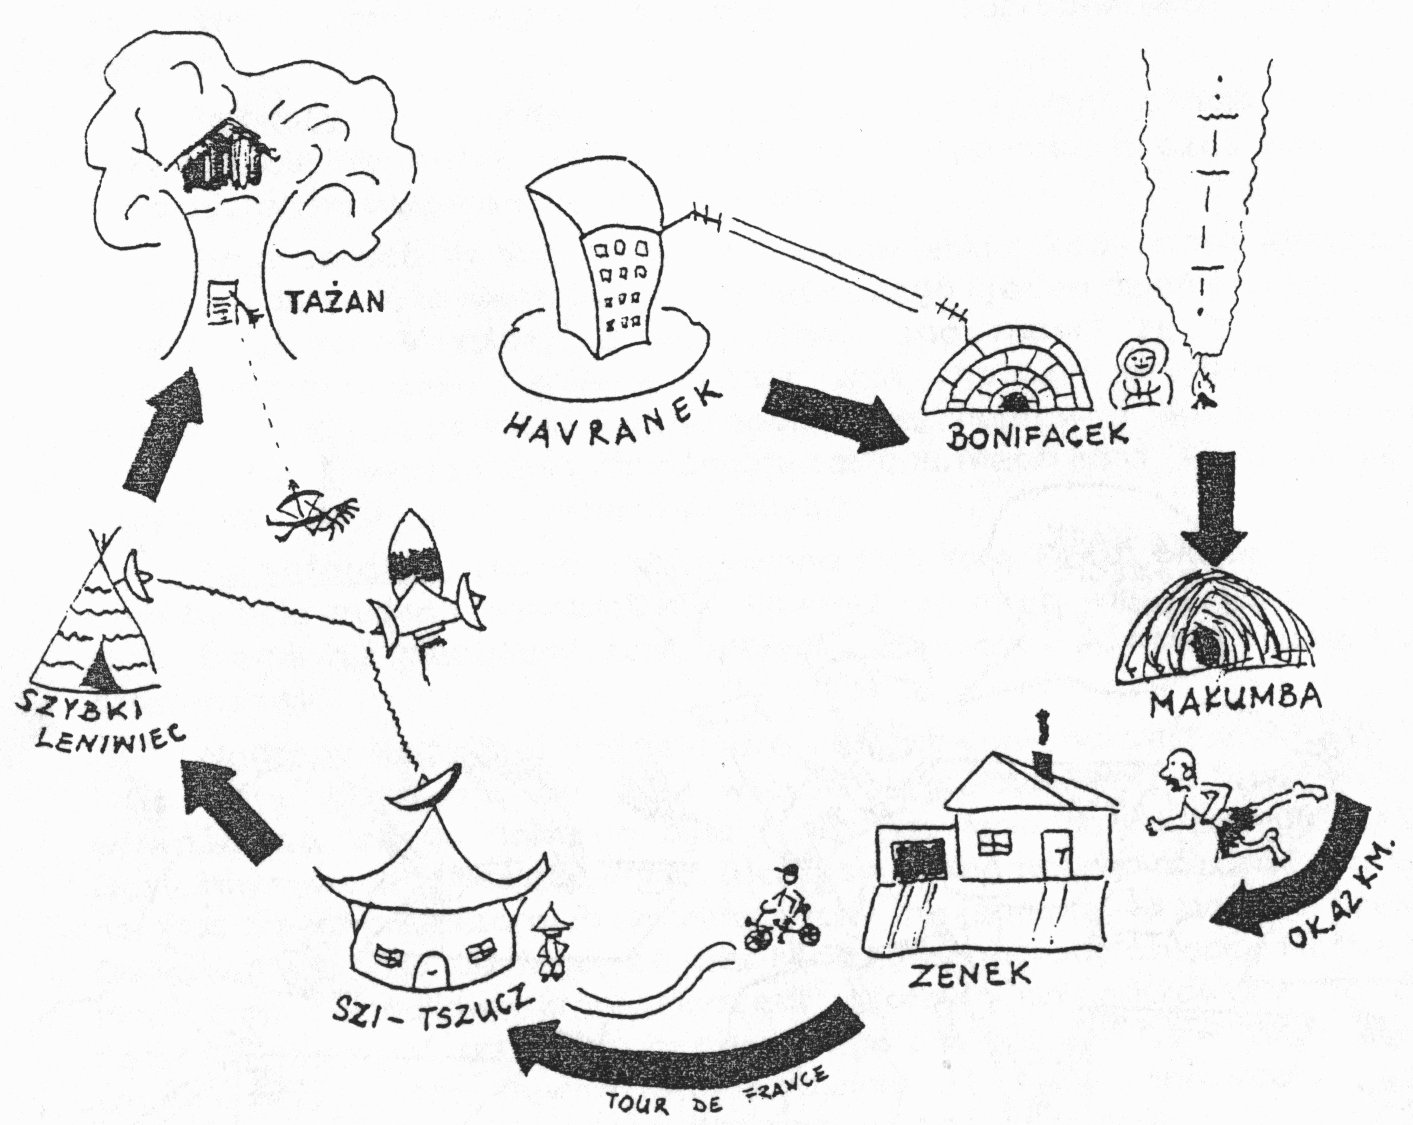
\includegraphics[width=0.5\textwidth]{grafiki/siec.png}
\end{center}
\end{figure}


\section{Zastęp na obozie}
To najlepszy okres w pracy zastępu. Dlaczego? Bo cały zastęp jest razem, przez  24 godziny na dobę, przez niemal cały miesiąc. Podczas dobrze przygotowanego obozu z zastępem możesz zrobić więcej, niż przez cały rok dobrej pracy.
	Warunkiem podstawowym jest, by zastępowy jechał na obóz! Bo to zastępowy przekazuje swoje umiejętności i wyrobienie pozostałym harcerzom zastępu:

- chłopacy mogą nie umieć rozbić namiotu, rozpalić ogniska, oprawić młotka. Ale zastępowy? Powinieneś im to  pokazać i pomóc.

- chłopcy mogą nie umieć odpowiednio (jak na harcerzy przystało) zachować się. Ale zastępowy ? Ty powinieneś być wzorem godnym naśladowania. Twoi harcerze z zastępu obserwują i naśladują Cię dzień i noc. Jeżeli Ty nawalisz oni także!

- chłopcy mogą się czasem obijać lub lenić. Ale zastępowy? Jako zastępowemu nie przystoi Tobie leżeć na kocu i wydawać  polecenia. Pracuj z całym zastępem, bardziej niż inni harcerze.

- chłopcy mogą nie wiedzieć jak najlepiej pełnić służby. Ale zastępowy? Ty organizujesz  służby rozdzielasz zadania, planujesz warty Dąż  wraz  z całym  zastępem do tego by Wasze służby były najlepsze, wzorowe. Zależy to przede  wszystkim  od  Ciebie.

\subsection{Atmosfera  na  obozie}
	Dbaj o dobrą atmosferę. Problemy i konflikty są nieuniknione, rozwiązuj  je  sprawiedliwie. Niech uśmiech nie znika z  twarzy Twoich harcerzy, ale przede wszystkim z Twojej. Może warto wieczorem zrobić całym zastępem rachunek  sumienia (podsumowanie dnia) i wymieniać co było dobrze, a co było nie tak. Każdy może się wtedy  wypowiedzieć, przeprosić, pogodzić ...

\subsection{Obozowe imprezy}
	Jako  zastępowy - wódz  powinieneś  dbać, by  w  obozowych  zajęciach  i  imprezach  uczestniczył  cały  zastęp. Jeśli więc jest festiwal piosenki obozowej niech cały zastęp wymyśla i śpiewa piosenkę, a nie tylko jeden harcerz, czy Ty sam.

\subsection{Służba zastępu na obozie}
	Służba - warta  jest  zaszczytem. Nie można stosować jej jako kary. Jak  przebiegnie  służba  zależy  od  Ciebie  i oboźnego. To czy Twój  zastęp i czy pozostali harcerze będą  zadowoleni zależy  od tego, jak  ta służba będzie zorganizowana. A powinna być przeprowadzona  sprawnie i sprawiedliwie.
	
\textbf{SPRAWNIE}: Chłopcy muszą wiedzieć dlaczego i jakie mają obowiązki. Muszą  wiedzieć kiedy i jak pełnią wartę, kogo budzą, że nie wolno zejść  z  warty zanim nie przyjdzie zmiana. Trzeba też wytłumaczyć, jak się pełni wartę, a to już sprawa zastępowego. Pamiętaj  także o posiłku dla  wartownika, będzie mu bardzo przykro, jeśli nie  dostanie go  wcale albo dostanie zimny!

Sprawna służba w  kuchni to nie tylko punktualne posiłki, pięknie wyglądające,  pachnące  i  smaczne. To także czystość  w  kuchni, porządek w magazynie. Nie ma nic gorszego jak leżące wokół kuchni papiery, brudne gary, porozrzucane wszędzie drewno, obierki na ziemi!!! Postaw się od czasu, do czasu w roli inspekcji sanitarnej i wraz zastępem zrób generalny porządek. W  porządku  łatwiej  wszystko  znaleźć a więc  lepiej  i szybciej się  pracuje.

\textbf{SPRAWIEDLIWIE}: Nie  można dzielić zadań i wart tak aby mali dostawali najgorszą  robotę i najgorsze warty. Nie można też tylko popuszczać małym i robić z nich mamisynków. Twoją rolą jest by podział wart i zadań w trakcie służby był sprawiedliwy.

	Pamiętaj Druhu Zastępowy! Obóz to  wspaniała zabawa,  niesamowite przygody, wielkie przeżycia, służba która wcale nie musi być kulą u nogi. Bardzo dużo jednak zależy od Ciebie, jak to zorganizujesz. Pomóż oboźnemu i komendantowi, a obóz naprawdę może być świetny!
	Ja chociaż byłem oboźnym i komendantem obozów najlepiej wspominam te, na których byłem zastępowym!

\chapter{Stopnie i sprawności}
\section{Stopnie harcerskie}
\begin{wrapfigure}{l}{4cm}
  \begin{center}
    
\includegraphics[width=4cm]{grafiki/krzyz.png}
  \end{center}
\end{wrapfigure} 
Każdy z nas zdobywa stopnie. Od chwili gdy przychodzimy na pierwszą zbiórkę, zaczynamy mozolnie wspinać się po drabinie harcerskiego życia, zdobywając szczebel po szczeblu kolejne stopnie. Pokazują one nie tylko ile drogi za nami,  ale przede wszystkim są drogowskazami w marszu do szczytu  ideałów.
	Nasz stopień staje się tak prawie ważny jak imię i nazwisko (wszak wymawiane jednym tchem), starajmy się abyśmy mogli być  z  niego dumni! Kiedy dostanę Krzyż, czy stopień? To pytanie stawiane często starszym druhom przez nowych chłopców w drużynie.  Pamiętajmy Krzyża Harcerskiego, stopnia się nie dostaje, trzeba go zdobyć i bynajmniej nie gadaniem o nim, tylko dobrze przygotowaną i zrealizowaną próbą. Zdobywanie nowego stopnia możemy podzielić na kilka etapów.  Oto one :


1.
Harcerz  przychodzi  do  drużynowego  albo Kapituły stopni (jeśli taka działa w drużynie) i zgłasza swoją  chęć  zdobywania  stopnia. Oczywiście  ktoś może mu to podpowiedzieć,  ale to musi być jego decyzja

2.
Chłopiec  przez  okres  kilku  miesięcy  pracuje  nad  sobą,  w   myśl  wskazówek drużynowego  lub  opiekuna  stopnia, stara  się  dostosować do wymagań stopnia.

3.
Drużynowy  opiekun lub Kapituła stopni  po  ocenie poprzedniego  etapu, uzgadnia  z harcerzem próbę  składającą się  z  ok. 10  zadań obejmujących  różne  dziedziny. Próba  jest  bardzo indywidualna (tak  jak  nie  ma  dwóch Jarków  Wiśniewskich, tak  nie ma dwóch takich samych prób), jak  też  bardzo  konkretna (więc nie ma  zadań  w  stylu powiadomił kogoś  w  ważnej sprawie, ale  np. powiadomiłem  druha Jacka  o  biwaku w  dniu  10 X). Wielką pomocą jest tutaj książeczka z regulaminem stopni harcerskich, która na pewno ma twój drużynowy, a którą może by było warto, abyś posiadał. Tam możesz zaznajomić się z ideą stopnia i wymaganiami na jego zdobycie.

4.
Otwarcie  próby  ogłasza  drużynowy  rozkazem (dla stopni HO - hufcowy, a dla stopnia HR - komendant  Chorągwi), a może  być  zamknięta   z  wynikiem  pozytywnym lub  negatywnym. Próba  trwa  ok. 3 - 12  miesięcy.

5.
Ostatni etap to próba końcowa trwająca 1 do 3 dni. Jest to jakiś wyczyn pokazujący, że ten  harcerz  siłą  charakteru, duchem i zaradnością  udowodnił,  że  jest  wzorowym   np. wywiadowcą.
Zdobyty  stopień   przyznaje  drużynowy, hufcowy (ćwika  i   Harcerza Orlego) lub komendant  Chorągwi (Harcerza  Rzeczypospolitej).


\section{Sprawności harcerskie}


\begin{wrapfigure}{l}{3cm}
  \begin{center}
    
\includegraphics[width=3cm]{grafiki/sprawnosc.png}
  \end{center}
\end{wrapfigure} Zbliżamy się powoli do naszego szczytu Siula Grande. Zdobywanie sprawności, jest niezwykle ważnym elementem harcerskiej kariery. Oczywiście chodzi tu o karierę w  doskonaleniu  samego  siebie. Osobą, mającą nieoceniony wpływ na zdobywanie sprawności w Twojej drużynie masz Ty Druhu Zastępowy. Nie każdy harcerz, od razu wpadnie na pomysł jaką sprawność może zdobyć. Nie każdy drużynowy, znajdzie tyle czasu, aby zajmować się wszystkim w drużynie. Dlatego Roland Philips wymyślił system zastępowy. To ty swoją służbą - Druhu  Zastępowy  pomagasz  zarówno harcerzom z zastępu jak i odciążasz drużynowego.

\noindent
	Zatem w przypadku zdobywania sprawności musisz: 

1. Wiedzieć co to jest sprawność.

2. Wiedzieć jak sprawność należy zdobywać.

3. Umieć przeprowadzić próbę na sprawność.

4. Posiadać własny egzemplarz regulaminu sprawności.

5. Znać go jak najlepiej.

Ad.1
Sprawność - jest to umiejętność, którą harcerz potwierdził  wykonując konkretne dzieło, zadanie. To musi  być  coś  porządnego. Podczas zdobywania sprawności nie ma czasu na naukę. Próba  sprawności jest swojego rodzaju egzaminem.

Ad. 2
Jak  zdobyć sprawność? Najpierw zapytaj samego siebie co chcesz zrobić? Najlepiej gdy Twój pomysł pasuje do realizowanego planu pracy drużyny, obozu, czy warunków  zewnętrznych. Trudno bowiem latem zdobyć sprawność Eskimosa. Po dokonaniu wyboru musisz  przeanalizować wymagania i nie przepisywać ich, tylko ułożyć konkretne zadania. Zadania te musi jeszcze zatwierdzić drużynowy lub Kapituła. Następnie  po  zatwierdzeniu najlepiej jak potrafisz wykonujesz zadania i już zdobyłeś sprawność. Teraz tylko rozkaz drużynowego i maksymalnie 3 dni na wyszycie sprawności na rękawie munduru! To  wszystko dotyczy Ciebie. Jeżeli sprawność zdobywa harcerz z Twojego zastępu, Ty  wiedząc więcej powinieneś mu  pomóc w dojściu do otwarcia próby. Dalej jednak musi sobie radzić sam.

Ad. 3
Jako zastępowy możesz mieć powierzone  przeprowadzenie części, a nawet całej  próby. Pamiętaj, że sprawność zdobywa się konkretnym działaniem, a nie gadaniem. W takiej sytuacji trzeba być bardzo konsekwentnym i wymagającym. Taką postawę trzeba  jednak łączyć  z  życzliwością! Pamiętaj, że sprawności przestają być atrakcyjne zarówno gdy próby  są zbyt trudne  jak  i  wtedy gdy próby  są  zbyt  łatwe.

Ad. 4
Jeżeli jeszcze nie masz Regulaminu sprawności, to natychmiast zażądaj od drużynowego, by ułatwił Ci kupienie go.

Ad. 5
Zanim zaczniesz wymądrzać się na temat zdobywania sprawności, przeczytaj kilka razy regulamin (całość ze wstępem i komentarzem!).

I jeszcze jedno\ldots Pamiętaj, że jako zastępowy powinieneś mieć kilka krążków więcej na rękawie munduru, niż inni harcerze z zastępu. Pomagając innym zdobywać sprawności, nie zapominaj o swoich próbach!

Oto wymagania na dwie sprawności  jednogwiazdkowe. Spróbuj w oparciu o te wymagania ułożyć zadania do próby.
\paragraph{Łącznik:}	\begin{itemize}[noitemsep,nolistsep] 
\item  bezbłędnie  przekazał ustny meldunek lub rozkaz złożony z kilkunastu słów
 \item zaadresował  list z użyciem kodu pocztowego, wypełnił blankiet telegramu, listu  poleconego, przekazu pieniężnego
\item  zapisał wiadomość korzystając z szyfru lub alfabetu Morse’a
\item  pełnił służbę łącznika w trakcie gry terenowej, zwiadu, wycieczki, okolicznościowej uroczystości.
\end{itemize}
\paragraph{Sobieradek obozowy:}	\begin{itemize}[noitemsep,nolistsep] 
\item  zaprojektował i wykonał drobny przedmiot pionierki obozowej (drogowskaz,  ławka,  wieszak, itp.)
\item  przygotował teren pod ognisko, ułożył  je i zamaskował po nim teren
\item  w pracach pionierskich  posłużył  się: piłą, toporkiem, młotkiem, potrafi je zakonserwować po skończonej pracy
\item  wraz z zastępem wykonał wnętrze swojego namiotu
\item  w pracach pionierskich posługiwał się swoimi wymiarami (rozstaw palców długość od końca dłoni do końca łokcia itp.)
\item  rozbił samodzielnie namiot  dwuosobowy, a z zastępem dziesięcioosobowy, w razie czego okopał go.
\item  wykazał umiejętności pionierskie stosując węzły
\end{itemize}
\chapter{Techniki harcerskie}
Z powodu ograniczonego miejsca, ten rozdział jest bardzo ogólnikowy.
\section{Terenoznawstwo}

Orientacja w terenie jest jedną z ważniejszych umiejętności jaką powinien posiadać każdy harcerz. Orientowanie się w terenie oprócz umiejętności zorientowania mapy ułatwia również obserwacja zjawisk przyrody. 
\paragraph{Sposoby orientacji w terenie}
\begin{description}[noitemsep,nolistsep] 

\item[Według położenia słońca] --- polega na ustawieniu się w słoneczny dzień w południe tyłem do słońca i zorientowaniu wg zasady że nasz cień pokazuje południe
\item[Według słońca i zegarka] --- jest to dość dokładna metoda ---- małą wskazówkę zegarka kierujemy ku słońcu. 
Teraz kąt między wskazówką, a cyfrą 12 dzielimy na połowę. Linia podziału wskazuje kierunek południowy (o 12:00). 
Pamiętać trzeba, że przed południem bierzemy pod uwagę kąt między małą wskazówką, a godz. 12. Po południu kąt między linią na godzinę 12, a małą wskazówkę
\item[Według gwiazdy polarnej] --- znajdujemy najpierw Wielki Wóz, a następnie przeprowadzamy przez dwie skrajne gwiazdy prostej, na której okładamy 5-krotną odległość między tymi gwiazdami. 
Na końcu tego odcinka znajduje się Gwiazda polarna wyznaczająca północ.
\item[W starych kościołach] ołtarze skierowane są w kierunku wschodnim.

\end{description}
\paragraph{Skala mapy}

Skala mapy informuje nas ile razy dana mapa została pomniejszona. Jak obliczyć jaka odległość na mapie odpowiada jakiej odległości w rzeczywistości? Jest to szalenie proste wystarczy z danej skali, np. 1:100000 skreślić 5 ostatnich cyfr. Wyjdzie nam wtedy, że 1 cm. na mapie odpowiada 1 km. w rzeczywistości. Szczegółowe mapy w Poznaniu można kupić na ul. Hawelańskiej 10 w Wojewódzkim Ośrodku Dokumentacji i Kartografii. Świetne mapy są dostępne także na stronie projektu http://geoportal.gov.pl

\paragraph{Mierzenie w terenie}

W terenie znajdują się różne rzeczy, których normalny śmiertelnik nie jest w stanie zmierzyć. No ale jako ze my jesteśmy harcerzami i dajemy sobie radę w wielu sytuacjach, to i w tym wypadku nie będzie to dla nas problem.

Pomiar szerokości rzeki - wbijamy krótką tyczkę na brzegu rzeki, i oddalamy się od niej z laską skautową na taka odległość, żeby z końca laski widzieć równocześnie koniec tyczki i krawędź drugiego brzegu.

Teraz za pomocą wzoru obliczamy szerokość rzeki: $AB= (DE x BD)/EF$
\begin{figure}[h]
\begin{center}
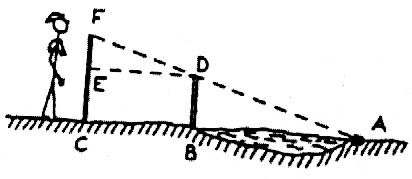
\includegraphics[width=0.7\textwidth]{grafiki/rzeka.png}
\end{center}
\end{figure}

2) Pomiar wysokości drzewa - sposób 1. 
Jeden z harcerzy zaznacza na lasce wyraźnie swoją wysokość od stóp do poziomu oczu, potem kładzie się na ziemi na wznak w odległości od podstawy drzewa przypuszczalnie równej wysokości drzewa. 
Drugi trzyma laskę pionowo przy jego stopach. 
Leżący przesuwa się na ziemi tak długo, aż znajdzie punkt, z którego przez miejsce zaznaczone na lasce zobaczy wierzchołek drzewa. 
Zmierzona ilość kroków od oka leżącego do podstawy drzewa na metry jest wysokością drzewa.
\begin{figure}[h]
\begin{center}
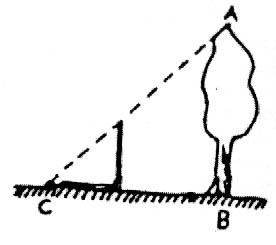
\includegraphics[width=0.3\textwidth]{grafiki/pomiardrzewa.png}
\end{center}
\end{figure}

3) Pomiar wysokości drzewa - sposób 2. Jeden z harcerzy staje pod drzewem. 
Drugi bierze kijek i stając w pewnej odległości przy wyciągniętej ręce z kijkiem zaznacza na nim wysokość harcerza. 
Następnie przy tej samej odległości i takim samym wyciągnięciu ręki mierzy kijkiem wysokość drzewa. 
Otrzymaną wysokość drzewa dzieli przez wysokość harcerza. 
Otrzymaną liczbę trzeba już tylko pomnożyć prze rzeczywisty wzrost harcerza.

\section{Łączność}
\begin{wrapfigure}{l}{3cm}
  \begin{center}
    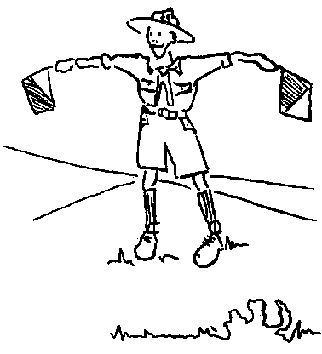
\includegraphics[width=3cm]{grafiki/lacznik.png}
  \end{center}
\end{wrapfigure} Łączność To bardzo rozległa dziedzina. 
Nie jest to wbrew pozorom tylko alfabet Morse’a i kilka innych szyfrów. 
Łączność to komunikacja międzyludzka za pomocą różnego rodzaju urządzeń i szyfrów. 
Do łączności zaliczają się więc m.in. : wysyłanie e-maili, rozmowa telefoniczna, łączność krótkofalarska, rozmowa za pomocą alfabetu Morse’a czy przekazywanie sobie nawzajem zaszyfrowanych wiadomości. 
	
\textbf{Alfabet Morse’a}
W 1837 roku niejaki Samuel Finley Breese Morse wynalazł telegraf elektromagnetyczny, a w 1840 stworzył dla niego specjalny alfabet telegraficzny zwany właśnie alfabetem Morse’a. 
Dzięki temu można było na duże odległości przekazywać sobie w krótkim czasie wiadomości, co było wcześniej niemożliwe. 
Obecnie alfabet Morse’a oprócz tego, że stosowany jest przez harcerzy, to wykorzystują go np. krótkofalowcy w łącznościach długodystansowych.

Alfabet ten składa się z kropek i kresek, które ułożone w odpowiedniej kolejności tworzą daną literę alfabetu. 
Żeby łatwiej było szyfrować i odczytywać wiadomości istnieje taka zasada: do każdej litery alfabetu przyporządkowywany jest odpowiedni wyraz, który dzielimy na sylaby. 
Jeśli w danej sylabie znajduje się „o” to piszemy kreskę, w przeciwnym razie kropkę.


\section{Szyfry}

Szyfr ułamkowy:
Jest to prosty szyfr. Alfabet dzielimy na poszczególne grupy i każdej takiej grupie przyporządkowujemy kolejno mianownik: 1, 2, 3, 4, 5. Potem przy zapisie w liczniku piszemy numer porządkowy danej litery, a mianownik przepisujemy. Litery i wyrazy można łączyć dowolnymi znakami matematycznymi\ldots
\begin{figure}[h]
\begin{center}
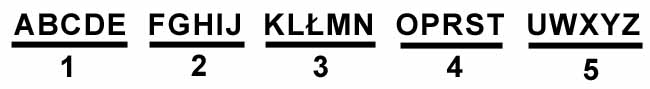
\includegraphics[width=0.9\textwidth]{grafiki/ulamkowy1.png}
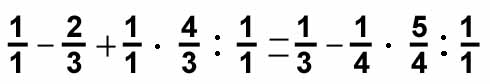
\includegraphics[width=0.9\textwidth]{grafiki/ulamkowy2.png}
\end{center}
\end{figure}



Szyfr ramowy/czekoladka:
\begin{figure}[h]
\begin{center}
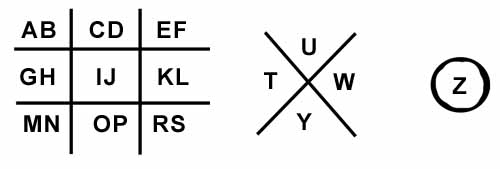
\includegraphics[width=0.9\textwidth]{grafiki/czekoladka.png}
\end{center}
\end{figure}

\paragraph{Pozostałe szyfry:}
Bardzo popularne szyfry takie jak GA-DE-RY PO-LU-KI, dzielimy go na sylaby, a następnie każdą literę, którą mamy zamienić zamieniamy na tę obok. Jeśli w szyfrze nie ma takiej litery, to ją normalnie przepisujemy. Istnieją też inne szyfry działające na tej samej zasadzie, takie jak: KONIEC MATURY, DALEKO TURYNI, KACE MINUTOWY, czy POLITYKA RENU.

\paragraph{Stwórz szyfr zastępu} --- tak by nikt inny nie mógł odczytywać Waszych wiadomości.





\chapter{Biblioteczka zastępowego}
\begin{wrapfigure}{l}{4cm}
  \begin{center}
    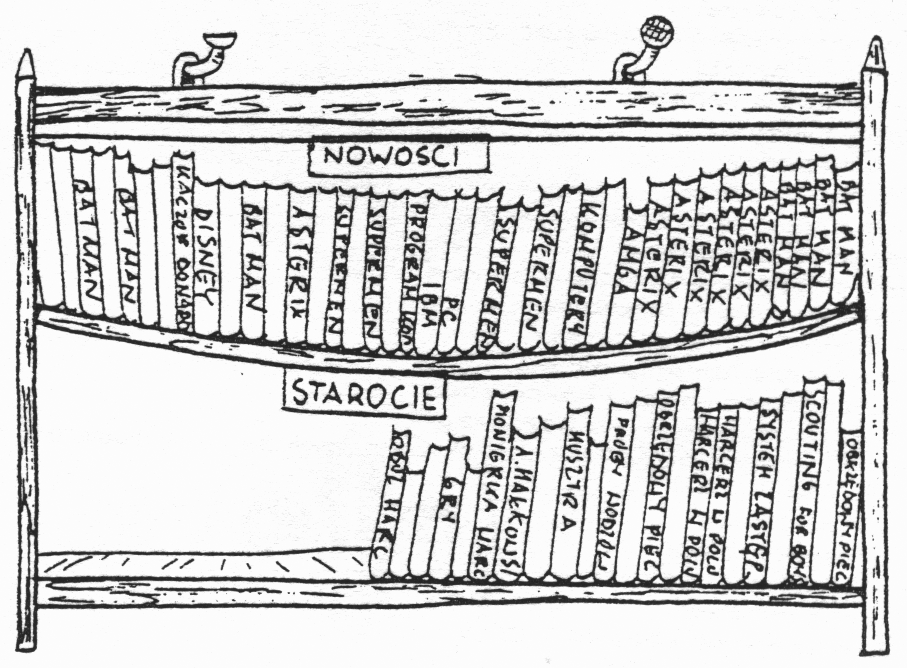
\includegraphics[width=4cm]{grafiki/biblioteczka.png}
  \end{center}
\end{wrapfigure} Spis ten nie wyczerpuje wszystkich pozycji przydatnych zastępowemu, do tej listy dołączyć należałoby wiele innych książek o tematyce historycznej, przygodowej, krajoznawczej. W biblioteczce zastępowego powinno być miejsce także dla śpiewników, map, czasopism, wydawnictw okazjonalnych itp. Biblioteka zastępowego to kopalnia pomysłów na zbiórki, wyprawy... Pamiętajcie jednak by nie zżynać dokładnie z książek, twórzcie w oparciu o to co przeczytaliście nowe, lepsze, ciekawsze formy pracy!
\begin{multicols}{2}
\begin{itemize}[noitemsep,nolistsep] 
\small
\item	R. Baden-Powell - Skauting dla chłopców
\item	R. Baden-Powell – Wskazówki dla skautmistrzów
\item	W. Błażejewski - Z dziejów harcerstwa polskiego
\item	A. Chmielewski - Tropy i ślady zwierząt
\item	M. Cmielowa - Wykapka
\item	J. Dąbrowski - Gry i zabawy w izbie harcerskiej
\item	J. Dąbrowski - Harce zimowe
\item	J. Dąbrowski - W świetlicy harcerskiej
\item	J. Dąbrowski i T. Kwiatkowski - Jeden trudny rok
\item	A. Dziewanowska, K. Rejs i Z. Zakrzewska - Gry i ćwiczenia w zastępie harcerskim
\item	S. Gawkowski - Szkice polowe harcerza
\item	E. Grodecka i J. Zwolakowska - Ćwiczenia i gry
\item	A. Gromski - Harce młodzika i wywiadowcy
\item	W. Hansen – Wilk, który nigdy nie śpi
\item	J. Jasiński - Gry i ćwiczenia terenowe
\item	A. Kamiński - A. Małkowski
\item	A. Kamiński - Kamienie na szaniec
\item	A. Kamiński - Zośka i Parasol
\item	M. Kapiszewska - Księga Harców R.Philips - System zastępowy
\item	A. Kazanecki - Terenoznawstwo dla harcerzy
\item	A. Kazanecki - Z notatnikiem i busolą - zbiór gier
\item	B. Kowalska i A. Kiewicz - Eskimos (materiały do zbiórek)
\item	M. Kudasiewicz - Obrzędowy piec
\item	T. Kwiatkowski - Obrzędy harcerskie
\item	O. Małkowska - A. Małkowski
\item	O. Nassalski - Jak pracować nad charakterem
\item	W. Nekrasz - Pionierka harcerska
\item	J. Parzyński - Obóz harcerski
\item	A. Pawełek - Młoda drużyna
\item	W. Pijanowski - Rozkosze łamania głowy
\item	W. Pijanowski - Skarbnica gier
\item	St. Sedlaczek - Drogowskaz Harcerza
\item	St. Sedlaczek - Geneza skautingu i harcerstwa
\item	St. Słysz - Gry i zabawy
\item	St. Sosnowski i J. Stykowski - Sakwa włóczykija
\item	W. Śliwerski - Harcerskie biegi
\item	J. Stykowski - Na traperskiej ścieżce
\item	J. Stykowski - Wyspa Robinsona
\item	J. Stykowski - Zastęp zbiórka (cykl 4 częściowy: wiosna, lato, jesień, zima)
\item	W. Szczygieł - Jak prowadzić zastęp harcerski
\item	W. Szyrzyński - Ambulans harcerski
\item	W. Szyrzyński - Wycieczki harcerskie
\item	Z. Trylski - Mały podręcznik obozowania
\item	Z. Trylski - Obozy 
\item	L. Ungeheuer - Próby wodzów
\item	B. Wachowicz – Wierna rzeka harcerstwa
\item	M. Wardęcki - Harcerskie gry terenowe
\item	A. Wasilewski - Pod totemem słońca
\item	P. Wieczorek – Wzgórze rosiczki
\item	R. M. Wujek - Skauting dzisiaj (gawędy o harcerstwie)
\item	Z. Wyrobek - Vademecum skauta
\item	Z. Wyrobek - Harcerz w polu
\item	http://www.zhr.pl/
\item	http://www.zastepowy.zhr.pl/
\end{itemize}
\end{multicols}

\chapter{Autorzy treści}

Marcin Gmerek ćw., 
pwd. Szymon Fiedler HO, 
pwd. Krzysztof Firlik HO, 
phm. Maciej Kaczmarek HO, 
pwd. Jarosław Kowalski HO, 
hm. Tomasz Łęcki HR, 
phm. Tomasz Nowacki HO, 
Marcin Rozmiarek ćw., 
phm. Jarosław Wagner HR, 
o. pwd. Marcin Wrzos HR 
i pwd. Wacław Łuczak HO
Alfa Tester



%\bibliographystyle{plain}
%\bibliography{bibliography}
\end{document}